%!TEX program = xelatex
% Encoding: UTF8
% SEIKA 2015

%\documentclass[a4paper,11pt,twoside]{book}
\documentclass[a4paper,11pt,twoside]{ctexbook}

\usepackage{geometry}
\geometry{left=3.5cm, right=3cm, top=3cm, bottom=3cm}
%控制页眉页脚页码
\pagestyle{headings}
%罗马字符页码
%\pagenumbering{roman}

%\usepackage{ctex}    uncomment this if article is applied on docclass
%\usepackage{xeCJK}   uncomment this if article is applied on docclass

%\CJKsetecglue{} % 禁用汉字与其他内容之间空格(空隙)
%\usepackage{ctex}

% 支持西文字体
\usepackage{fourier}
\usepackage{courier}
% \usepackage{fontspec}
\newfontfamily\CodeFont{Ubuntu Mono}

\usepackage{graphicx}
% 支持插入eps图形文件
% \usepackage{epsfig}

% 支持超链接
\usepackage[colorlinks]{hyperref}

% 支持代码框插入
\usepackage{xcolor}
\definecolor{mygreen}{rgb}{0,0.6,0}
\definecolor{mygray}{rgb}{0.5,0.5,0.5}
\definecolor{mymauve}{rgb}{0.58,0,0.82}
\definecolor{myback}{rgb}{0.95,0.95,0.95}

\usepackage{listings}
\lstset{ %
  backgroundcolor=\color{myback},    % choose the background color; you must add \usepackage{color} or \usepackage{xcolor}
  basicstyle=\linespread{0.99}\small  \CodeFont,   % the size of the fonts that are used for the code
  breakatwhitespace=false,           % sets if automatic breaks should only happen at whitespace
  breaklines=true,                   % sets automatic line breaking
  captionpos=bl,                     % sets the caption-position to bottom
  commentstyle=\color{mygreen},      % comment style
  deletekeywords={...},              % if you want to delete keywords from the given language
  escapeinside={\%*}{*)},            % if you want to add LaTeX within your code
  extendedchars=true,                % lets you use non-ASCII characters; for 8-bits encodings only, does not work with UTF-8
  frame=single,                      % adds a frame around the code
  keepspaces=true,                   % keeps spaces in text, useful for keeping indentation of code (possibly needs columns=flexible)
  keywordstyle=\color{blue},         % keyword style
  language=Python,                   % the language of the code
  morekeywords={*,...},              % if you want to add more keywords to the set
  numbers=left,                      % where to put the line-numbers; possible values are (none, left, right)
  numbersep=4pt,                     % how far the line-numbers are from the code
  numberstyle=\tiny\CodeFont\color{mygray},   % the style that is used for the line-numbers
  rulecolor=\color{mygray},          % if not set, the frame-color may be changed on line-breaks within not-black text (e.g. comments (green here))
  showspaces=false,                  % show spaces everywhere adding particular underscores; it overrides 'showstringspaces'
  showstringspaces=true,             % underline spaces within strings only
  showtabs=true,                     % show tabs within strings adding particular underscores
  stepnumber=1,                      % the step between two line-numbers. If it's 1, each line will be numbered
  stringstyle=\color{orange},        % string literal style
  tabsize=2,                         % sets default tabsize to 2 spaces
  %title=myPython.py                 % show the filename of files included with \lstinputlisting; also try caption instead of title
}

% \setCJKmainfont[BoldFont={SimSun},ItalicFont={KaiTi}] %{SimSun}

%%%%%%%%%%%%
\title{Tensorflow 指南}
\author{}
\date{2015-12-16}
% \thanks{}

\begin{document}

\maketitle
\newpage
\tableofcontents
\newpage

\chapter{起步}
% \section{Introduction}
\section{Introduction}
Let's get you up and running with TensorFlow!

But before we even get started, let's peek at what TensorFlow code looks like in the Python API, so you have a sense of where we're headed.

Here's a little Python program that makes up some data in two dimensions, and then fits a line to it.

\begin{lstlisting}
import tensorflow as tf
import numpy as np

# Create 100 phony x, y data points in NumPy, y = x * 0.1 + 0.3
x_data = np.random.rand(100).astype("float32")
y_data = x_data * 0.1 + 0.3

# Try to find values for W and b that compute y_data = W * x_data + b
# (We know that W should be 0.1 and b 0.3, but Tensorflow will
# figure that out for us.)
W = tf.Variable(tf.random_uniform([1], -1.0, 1.0))
b = tf.Variable(tf.zeros([1]))
y = W * x_data + b

# Minimize the mean squared errors.
loss = tf.reduce_mean(tf.square(y - y_data))
optimizer = tf.train.GradientDescentOptimizer(0.5)
train = optimizer.minimize(loss)

# Before starting, initialize the variables.  We will 'run' this first.
init = tf.initialize_all_variables()

# Launch the graph.
sess = tf.Session()
sess.run(init)

# Fit the line.
for step in xrange(201):
    sess.run(train)
    if step % 20 == 0:
        print(step, sess.run(W), sess.run(b))

# Learns best fit is W: [0.1], b: [0.3]
\end{lstlisting}

The first part of this code builds the data flow graph. TensorFlow does not actually run any computation until the session is created and the run function is called.

To whet your appetite further, we suggest you check out what a classical machine learning problem looks like in TensorFlow. In the land of neural networks the most "classic" classical problem is the MNIST handwritten digit classification. We offer two introductions here, one for machine learning newbies, and one for pros. If you've already trained dozens of MNIST models in other software packages, please take the red pill. If you've never even heard of MNIST, definitely take the blue pill. If you're somewhere in between, we suggest skimming blue, then red.

% Add pics and links here

If you're already sure you want to learn and install TensorFlow you can skip these and charge ahead. Don't worry, you'll still get to see MNIST -- we'll also use MNIST as an example in our technical tutorial where we elaborate on TensorFlow features.

Recommended Next Steps

Download and Setup
Basic Usage
TensorFlow Mechanics 101

本章的目的是让你了解和运行 TensorFlow!

在开始之前, 让我们先看一段使用 Python API 撰写的 TensorFlow 示例代码,
让你对将要学习的内容有初步的印象.

这段很短的 Python 程序生成了一些三维数据, 然后用一个平面拟合它.

\begin{lstlisting}
import tensorflow as tf
import numpy as np

# 使用 NumPy 生成假数据(phony data), 总共 100 个点.
x_data = np.float32(np.random.rand(2, 100)) # 随机输入
y_data = np.dot([0.100, 0.200], x_data) + 0.300

# 构造一个线性模型
#
b = tf.Variable(tf.zeros([1]))
W = tf.Variable(tf.random_uniform([1, 2], -1.0, 1.0))
y = tf.matmul(W, x_data) + b

# 最小化方差
loss = tf.reduce_mean(tf.square(y - y_data))
optimizer = tf.train.GradientDescentOptimizer(0.5)
train = optimizer.minimize(loss)

# 初始化变量
init = tf.initialize_all_variables()

# 启动图 (graph)
sess = tf.Session()
sess.run(init)

# 拟合平面
for step in xrange(0, 201):
    sess.run(train)
    if step % 20 == 0:
        print step, sess.run(W), sess.run(b)

# 得到最佳拟合结果 W: [[0.100  0.200]], b: [0.300]
\end{lstlisting}

为了进一步激发你的学习欲望, 我们想让你先看一下 TensorFlow 是如何解决一个经典的机器学习问题的. 在神经网络领域, 最为经典的问题莫过于 MNIST 手写数字分类问题. 我们准备了两篇不同的教程, 分别面向机器学习领域的初学者和专家. 如果你已经使用其它软件训练过许多MNIST 模型, 请阅读高级教程 (红色药丸链接). 如果你以前从未听说过 MNIST, 请阅读初级教程(蓝色药丸链接). 如果你的水平介于这两类人之间, 我们建议你先快速浏览初级教程, 然后再阅读高级教程.

% <div style="width:100%; margin:auto; margin-bottom:10px; margin-top:20px; display: flex; flex-direction: row">
%  <a href="tensorflow-zh/SOURCE/tutorials/mnist_beginners.md" title="面向机器学习初学者的 MNIST 初级教程">
%    <img style="flex-grow:1; flex-shrink:1; border: 1px solid black;" src="../images/blue_pill.png" alt="面向机器学习初学者的 MNIST 初级教程" />
%  </a>
%  <a href="tensorflow-zh/SOURCE/tutorials/mnist_pros.md" title="面向机器学习专家的 MNIST 高级教程">
%    <img style="flex-grow:1; flex-shrink:1; border: 1px solid black;" src="../images/red_pill.png" alt="面向机器学习专家的 MNIST 高级教程" />
%  </a>
% </div>
% <p style="font-size:10px;">图片由 CC BY-SA 4.0 授权; 原作者 W. Carter</p>

如果你已经下定决心, 准备学习和安装 TensorFlow, 你可以略过这些文字, 直接阅读
后面的章节. 不用担心, 你仍然会看到 MNIST -- 在阐述 TensorFlow 的特性时,
我们还会使用 MNIST 作为一个样例.

% ## 推荐随后阅读: <a class="md-anchor" id="AUTOGENERATED-recommended-next-steps-"></a>%

% * [下载与安装](../get_started/os_setup.md)
% * [基本使用](../get_started/basic_usage.md)
% * [TensorFlow 技术指南](../tutorials/mnist/tf/index.md)%

% <div class='sections-order' style="display: none;">
% <!-- os_setup.md -->
% <!-- basic_usage.md -->
% </div>%

% > 原文:[Introduction](http://tensorflow.org/get_started)  翻译:[@doc001](https://github.com/PFZheng)  校对:[@yangtze](https://github.com/sstruct)

\section{Download and Setup}

\newpage

\section{Basic Usage}

To use TensorFlow you need to understand how TensorFlow:

\begin{itemize}
\item Represents computations as graphs.
\item Executes graphs in the context of Sessions.
\item Represents data as tensors.
\item Maintains state with Variables.
\item Uses feeds and fetches to get data into and out of arbitrary operations.
\end{itemize}

\subsection{Overview}

TensorFlow is a programming system in which you represent computations as graphs. Nodes in the graph are called ops (short for operations). An op takes zero or more \lstinline{Tensors}, performs some computation, and produces zero or more \lstinline{Tensors}. A Tensor is a typed multi-dimensional array. For example, you can represent a mini-batch of images as a 4-D array of floating point numbers with dimensions \lstinline{[batch, height, width, channels]}.

\subsection{The computation graph}

TensorFlow programs are usually structured into a construction phase, that assembles a graph, and an execution phase that uses a session to execute ops in the graph.

For example, it is common to create a graph to represent and train a neural network in the construction phase, and then repeatedly execute a set of training ops in the graph in the execution phase.

TensorFlow can be used from C, C++, and Python programs. It is presently much easier to use the Python library to assemble graphs, as it provides a large set of helper functions not available in the C and C++ libraries.

The session libraries have equivalent functionalities for the three languages.

\subsubsection {Building the graph}
To build a graph start with ops that do not need any input (source ops), such as Constant, and pass their output to other ops that do computation.

The ops constructors in the Python library return objects that stand for the output of the constructed ops. You can pass these to other ops constructors to use as inputs.

The TensorFlow Python library has a default graph to which ops constructors add nodes. The default graph is sufficient for many applications. See the Graph class documentation for how to explicitly manage multiple graphs.

\begin{lstlisting}
import tensorflow as tf

# Create a Constant op that produces a 1x2 matrix.  The op is
# added as a node to the default graph.
#
# The value returned by the constructor represents the output
# of the Constant op.
matrix1 = tf.constant([[3., 3.]])

# Create another Constant that produces a 2x1 matrix.
matrix2 = tf.constant([[2.],[2.]])

# Create a Matmul op that takes 'matrix1' and 'matrix2' as inputs.
# The returned value, 'product', represents the result of the matrix
# multiplication.
product = tf.matmul(matrix1, matrix2)
\end{lstlisting}

The default graph now has three nodes: two constant() ops and one matmul() op. To actually multiply the matrices, and get the result of the multiplication, you must launch the graph in a session.

\subsubsection {Launching the graph in a session}

Launching follows construction. To launch a graph, create a Session object. Without arguments the session constructor launches the default graph.

See the Session class for the complete session API.

\begin{lstlisting}
# Launch the default graph.
sess = tf.Session()

# To run the matmul op we call the session 'run()' method, passing 'product'
# which represents the output of the matmul op.  This indicates to the call
# that we want to get the output of the matmul op back.
#
# All inputs needed by the op are run automatically by the session.  They
# typically are run in parallel.
#
# The call 'run(product)' thus causes the execution of threes ops in the
# graph: the two constants and matmul.
#
# The output of the op is returned in 'result' as a numpy `ndarray` object.
result = sess.run(product)
print(result)
# ==> [[ 12.]]

# Close the Session when we're done.
sess.close()
\end{lstlisting}

Sessions should be closed to release resources. You can also enter a Session with a "with" block. The Session closes automatically at the end of the with block.

\begin{lstlisting}
with tf.Session() as sess:
  result = sess.run([product])
  print(result)
\end{lstlisting}

The TensorFlow implementation translates the graph definition into executable operations distributed across available compute resources, such as the CPU or one of your computer's GPU cards. In general you do not have to specify CPUs or GPUs explicitly. TensorFlow uses your first GPU, if you have one, for as many operations as possible.

If you have more than one GPU available on your machine, to use a GPU beyond the first you must assign ops to it explicitly. Use with...Device statements to specify which CPU or GPU to use for operations:

\begin{lstlisting}
with tf.Session() as sess:
  with tf.device("/gpu:1"):
    matrix1 = tf.constant([[3., 3.]])
    matrix2 = tf.constant([[2.],[2.]])
    product = tf.matmul(matrix1, matrix2)
    ...
\end{lstlisting}

Devices are specified with strings. The currently supported devices are:

"/cpu:0": The CPU of your machine.
"/gpu:0": The GPU of your machine, if you have one.
"/gpu:1": The second GPU of your machine, etc.
See Using GPUs for more information about GPUs and TensorFlow.

\subsection{Interactive Usage}

\subsection{Tensors}
\subsection{Variables}
\subsection{Fetches}
\subsection{Feeds}

\begin{lstlisting}
\end{lstlisting}

\begin{lstlisting}
\end{lstlisting}

\begin{lstlisting}
\end{lstlisting}

\begin{lstlisting}
\end{lstlisting}



\newpage

%\chapter{基础教程}
%!TEX program = xelatex
% Encoding: UTF8
% SEIKA 2015


% Chapter 2 TutorialsHow to ...
% Section 2.1

\section{综述}

\textbf{MNIST For ML Beginners}

If you're new to machine learning, we recommend starting here. You'll learn about a classic problem, handwritten digit classification (MNIST), and get a gentle introduction to multiclass classification.

View Tutorial

\textbf{Deep MNIST for Experts}

If you're already familiar with other deep learning software packages, and are already familiar with MNIST, this tutorial with give you a very brief primer on TensorFlow.

View Tutorial

\textbf{TensorFlow Mechanics 101}

This is a technical tutorial, where we walk you through the details of using TensorFlow infrastructure to train models at scale. We use again MNIST as the example.

View Tutorial

\textbf{Convolutional Neural Networks}

An introduction to convolutional neural networks using the CIFAR-10 data set. Convolutional neural nets are particularly tailored to images, since they exploit translation invariance to yield more compact and effective representations of visual content.

View Tutorial

\textbf{Vector Representations of Words}

This tutorial motivates why it is useful to learn to represent words as vectors (called word embeddings). It introduces the word2vec model as an efficient method for learning embeddings. It also covers the high-level details behind noise-contrastive training methods (the biggest recent advance in training embeddings).

View Tutorial

\textbf{Recurrent Neural Networks}

An introduction to RNNs, wherein we train an LSTM network to predict the next word in an English sentence. (A task sometimes called language modeling.)

View Tutorial

\textbf{Sequence-to-Sequence Models}

A follow on to the RNN tutorial, where we assemble a sequence-to-sequence model for machine translation. You will learn to build your own English-to-French translator, entirely machine learned, end-to-end.

View Tutorial

\textbf{Mandelbrot Set}

TensorFlow can be used for computation that has nothing to do with machine learning. Here's a naive implementation of Mandelbrot set visualization.

View Tutorial

\textbf{Partial Differential Equations}

As another example of non-machine learning computation, we offer an example of a naive PDE simulation of raindrops landing on a pond.

View Tutorial

\textbf{MNIST Data Download}

Details about downloading the MNIST handwritten digits data set. Exciting stuff.

View Tutorial

\textbf{Image Recognition}

How to run object recognition using a convolutional neural network trained on ImageNet Challenge data and label set.

View Tutorial

We will soon be releasing code for training a state-of-the-art Inception model.

Deep Dream Visual Hallucinations

Building on the Inception recognition model, we will release a TensorFlow version of the Deep Dream neural network visual hallucination software.

COMING SOON
%!TEX program = xelatex
% Encoding: UTF8
% SEIKA 2015


% Chapter 2 TutorialsHow to ...
% Section 2.2

\newpage
\section {MNIST之机器学习入门}\label{MINIST_beginner}

% This tutorial is intended for readers who are new to both machine learning and TensorFlow. If you already know what MNIST is, and what softmax (multinomial logistic) regression is, you might prefer this faster paced tutorial. Be sure to install TensorFlow before starting either tutorial.

这个教程的目标读者是对机器学习和TensorFlow都不太了解的新手。如果你已经了解MNIST和softmax回归(softmax regression)的相关知识,你可以阅读这个快速上手教程。

% When one learns how to program, there's a tradition that the first thing you do is print "Hello World." Just like programming has Hello World, machine learning has MNIST.

当我们开始学习编程的时候,第一件事往往是学习打印“Hello World”。就好比编程入门有Hello World,机器学习入门有MNIST。
MNIST是一个入门级的计算机视觉数据集,它包含各种手写数字图片:
\begin{center}

\includegraphics[width=.55\textwidth]{../SOURCE/images/MNIST.png}
\end{center}
它也包含每一张图片对应的标签,告诉我们这个是数字几。比如,上面这四张图片的标签分别是5,0,4,1。

在此教程中,我们将训练一个机器学习模型用于预测图片里面的数字。我们的目的不是要设计一个世界一流的复杂模型 -- 尽管我们会在之后给你源代码去实现一流的预测模型 -- 而是要介绍下如何使用TensorFlow。所以,我们这里会从一个很简单的数学模型开始,它叫做Softmax Regression。

对应这个教程的实现代码很短,而且真正有意思的内容只包含在三行代码里面。但是,去理解包含在这些代码里面的设计思想是非常重要的:TensorFlow工作流程和机器学习的基本概念。因此,这个教程会很详细地介绍这些代码的实现原理。

\subsection {MNIST数据集}

MNIST数据集的官网是\href{http://yann.lecun.com/exdb/mnist/}{Yann LeCun's website}。在这里,我们提供了一份python源代码用于自动下载和安装这个数据集。你可以下载这段\href{https://tensorflow.googlesource.com/tensorflow/+/master/tensorflow/examples/tutorials/mnist/input_data.py}{代码},然后用下面的代码导入到你的项目里面,也可以直接复制粘贴到你的代码文件里面。

%\begin{lstlisting}[language={[ANSI]Python}]
\begin{lstlisting}
import input_data
mnist = input_data.read_data_sets("MNIST_data/", one_hot=True)
\end{lstlisting}

下载下来的数据集被分成两部分:60000行的训练数据集(`mnist.train`)和10000行的测试数据集(`mnist.test`)。这样的切分很重要,在机器学习模型设计时必须有一个单独的测试数据集不用于训练而是用来评估这个模型的性能,从而更加容易把设计的模型推广到其他数据集上(泛化)。

正如前面提到的一样,每一个MNIST数据单元有两部分组成:一张包含手写数字的图片和一个对应的标签。我们把这些图片设为“xs”,把这些标签设为“ys”。训练数据集和测试数据集都包含xs和ys,比如训练数据集的图片是\lstinline{mnist.train.images} ,训练数据集的标签是\lstinline{mnist.train.labels}。

每一张图片包含$ 28 \times 28$像素。我们可以用一个数字数组来表示这张图片:

\begin{center}
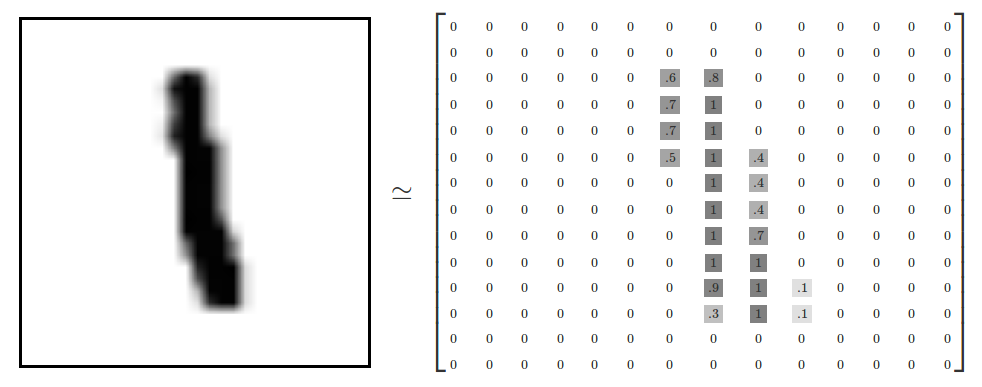
\includegraphics[width=.8\textwidth]{../SOURCE/images/MNIST-Matrix.png}
\end{center}

我们把这个数组展开成一个向量,长度是 $ 28 \times 28 = 784$。如何展开这个数组(数字间的顺序)不重要,只要保持各个图片采用相同的方式展开。从这个角度来看,MNIST数据集的图片就是在784维向量空间里面的点, 并且拥有比较复杂的结构 (提醒: 此类数据的可视化是计算密集型的)。

展平图片的数字数组会丢失图片的二维结构信息。这显然是不理想的,最优秀的计算机视觉方法会挖掘并利用这些结构信息,我们会在后续教程中介绍。但是在这个教程中我们忽略这些结构,所介绍的简单数学模型,softmax回归(softmax regression),不会利用这些结构信息。

因此,在MNIST训练数据集中,\lstinline{mnist.train.images}是一个形状为 [60000, 784] 的张量,第一个维度数字用来索引图片,第二个维度数字用来索引每张图片中的像素点。在此张量里的每一个元素,都表示某张图片里的某个像素的强度值,值介于0和1之间。

\begin{center}
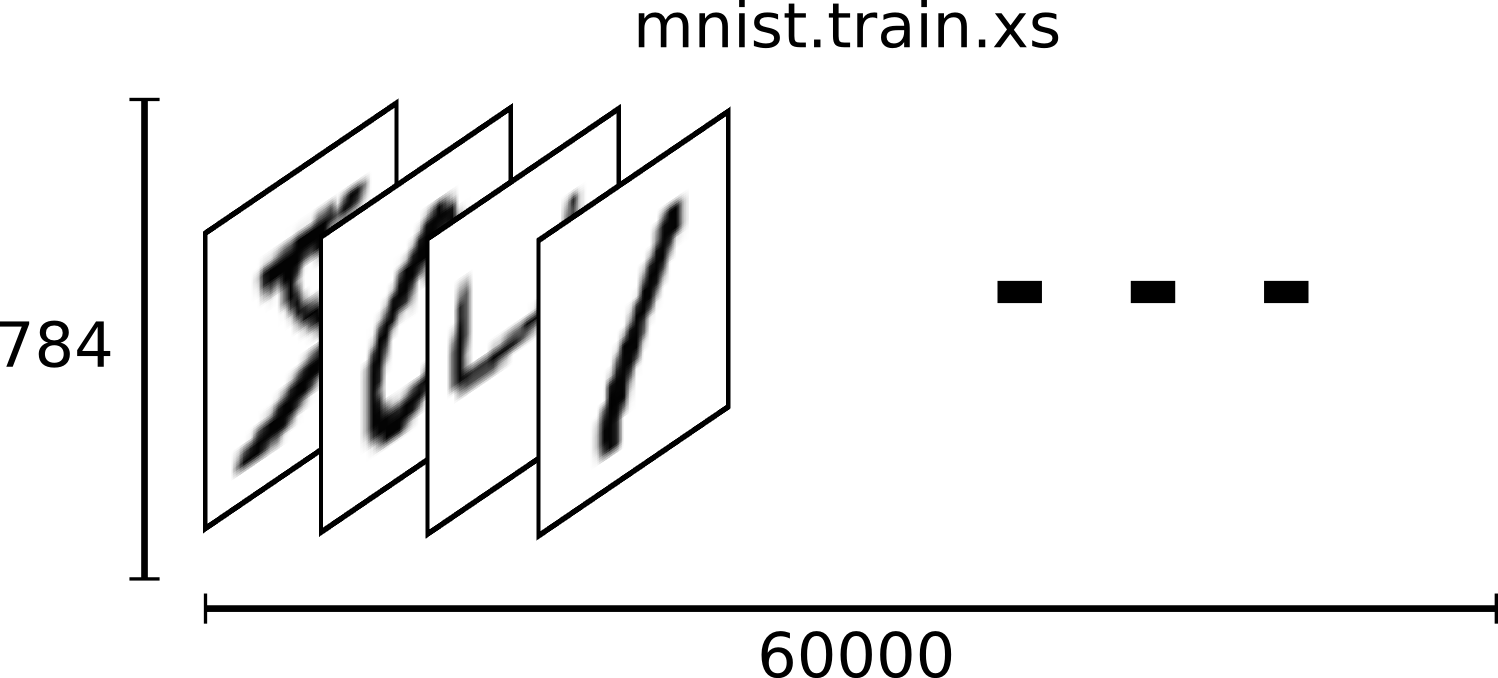
\includegraphics[width=.75\textwidth]{../SOURCE/images/mnist-train-xs.png}
\end{center}

相对应的MNIST数据集的标签是介于0到9的数字,用来描述给定图片里表示的数字。为了用于这个教程,我们使标签数据是"one-hot vectors"。 一个one-hot向量除了某一位的数字是1以外其余各维度数字都是0。所以在此教程中,数字n将表示成一个只有在第n维度(从0开始)数字为1的10维向量。比如,标签0将表示成([1,0,0,0,0,0,0,0,0,0,0])。因此,\lstinline{mnist.train.labels}是一个 [60000, 10] 的数字矩阵。

\begin{center}
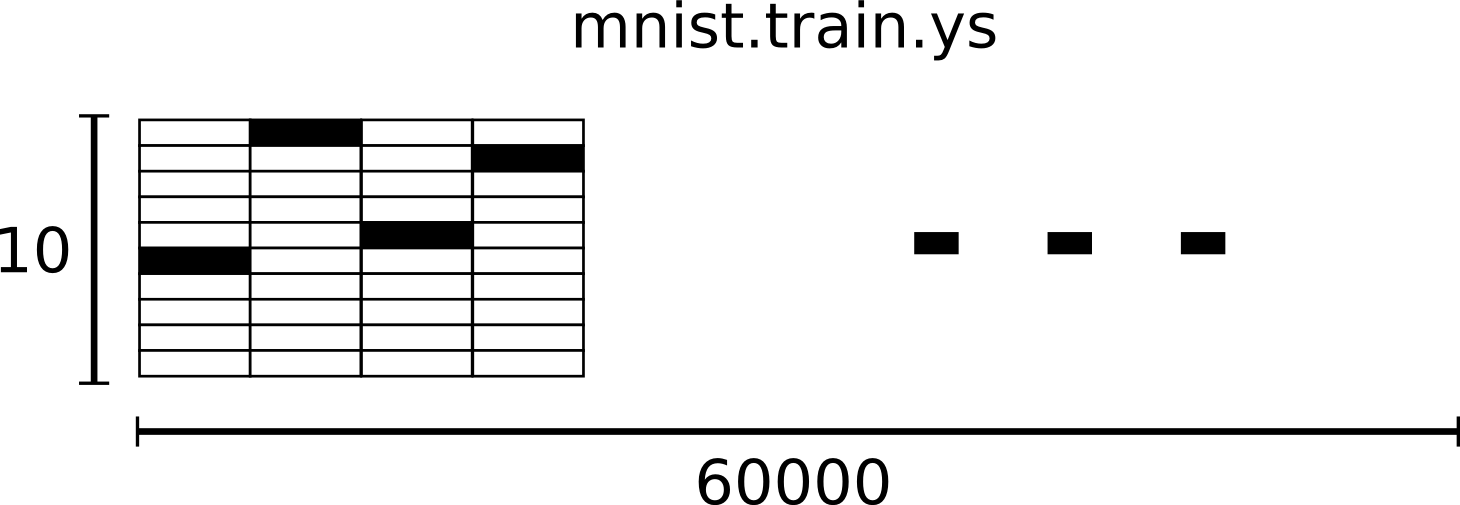
\includegraphics[width=.7\textwidth]{../SOURCE/images/mnist-train-ys.png}
\end{center}

现在,我们准备开始真正的建模之旅啦!

\subsection {Softmax回归介绍}

我们知道MNIST的每一张图片都表示一个数字,从0到9。我们希望得到给定图片代表每个数字的概率。比如说,我们的模型可能推测一张包含9的图片代表数字9的概率是80\%但是判断它是8的概率是5\%(因为8和9都有上半部分的小圆),然后给予它代表其他数字的概率更小的值。

这是一个使用softmax回归(softmax regression)模型的经典案例。softmax模型可以用来给不同的对象分配概率。即使在之后,我们训练更加精细的模型时,最后一步也需要用softmax来分配概率。

softmax回归(softmax regression)分两步:首先,为了得到一张给定图片属于某个特定数字类的证据(evidence),我们对图片像素值进行加权求和。如果这个像素具有很强的证据说明这张图片不属于该类,那么相应的权值为负数,相反如果这个像素拥有有利的证据支持这张图片属于这个类,那么权值是正数。
下面的图片显示了一个模型学习到的图片上每个像素对于特定数字类的权值。红色代表负数权值,蓝色代表正数权值。


\begin{center}
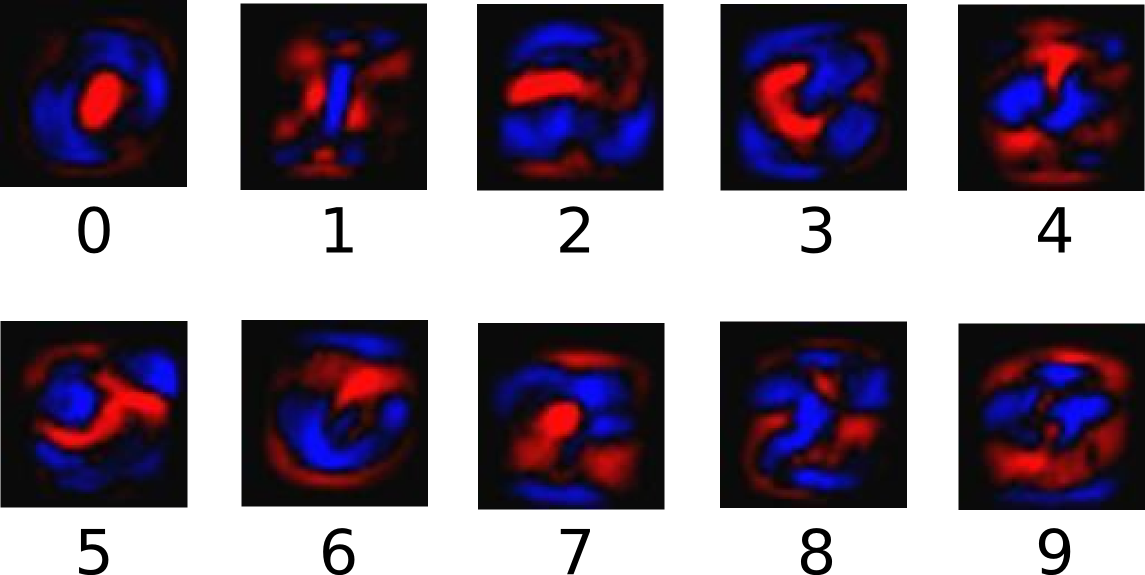
\includegraphics[width=.65\textwidth]{../SOURCE/images/softmax-weights.png}
\end{center}

我们也需要加入一个额外的偏置量(bias),因为输入往往会带有一些无关的干扰量。因此对于给定的输入图片$x$它代表的是数字$x$的证据可以表示为\\
\begin{equation}
evidence_i = \sum_j{W_{i,j}}x_j+b_i
\end{equation}\\
其中,$W_i$代表权重,$b_i$ 代表第$i$类的偏置量,$j$代表给定图片$x$的像素索引用于像素求和。然后用softmax函数可以把这些证据转换
成概率$y$:\\
\begin{equation}
y = softmax(evidence)
\end{equation}

这里的softmax可以看成是一个激励(activation)函数或是链接(link)函数,把我们定义的线性函数的输出转换成我们想要的格式,也就是关于10个数字类的概率分布。因此,给定一张图片,它对于每一个数字的吻合度可以被softmax函数转换成为一个概率值。softmax函数可以定义为:\\
\begin{equation}
softmax(x) = normalize(exp(x))
\end{equation}\\
展开等式右边的子式,可以得到:\\
\begin{equation}
softmax(x)_i = \frac{exp(x_i)}{\sum_j{exp(x_j)}}
\end{equation}\\
但是更多的时候把softmax模型函数定义为前一种形式:把输入值当成幂指数求值,再正则化这些结果值。这个幂运算表示,更大的证据对应更大的假设模型(hypothesis)里面的乘数权重值。反之,拥有更少的证据意味着在假设模型里面拥有更小的乘数系数。假设模型里的权值不可以是0值或者负值。Softmax然后会正则化这些权重值,使它们的总和等于1,以此构造一个有效的概率分布。(更多的关于Softmax函数的信息,可以参考Michael Nieslen的书里面的这个部分,其中有关于softmax的可交互式的可视化解释。)

对于softmax回归模型可以用下面的图解释,对于输入的$xs$ 加权求和,再分别加上一个偏置量,最后再输入到softmax函数中:
\begin{center}
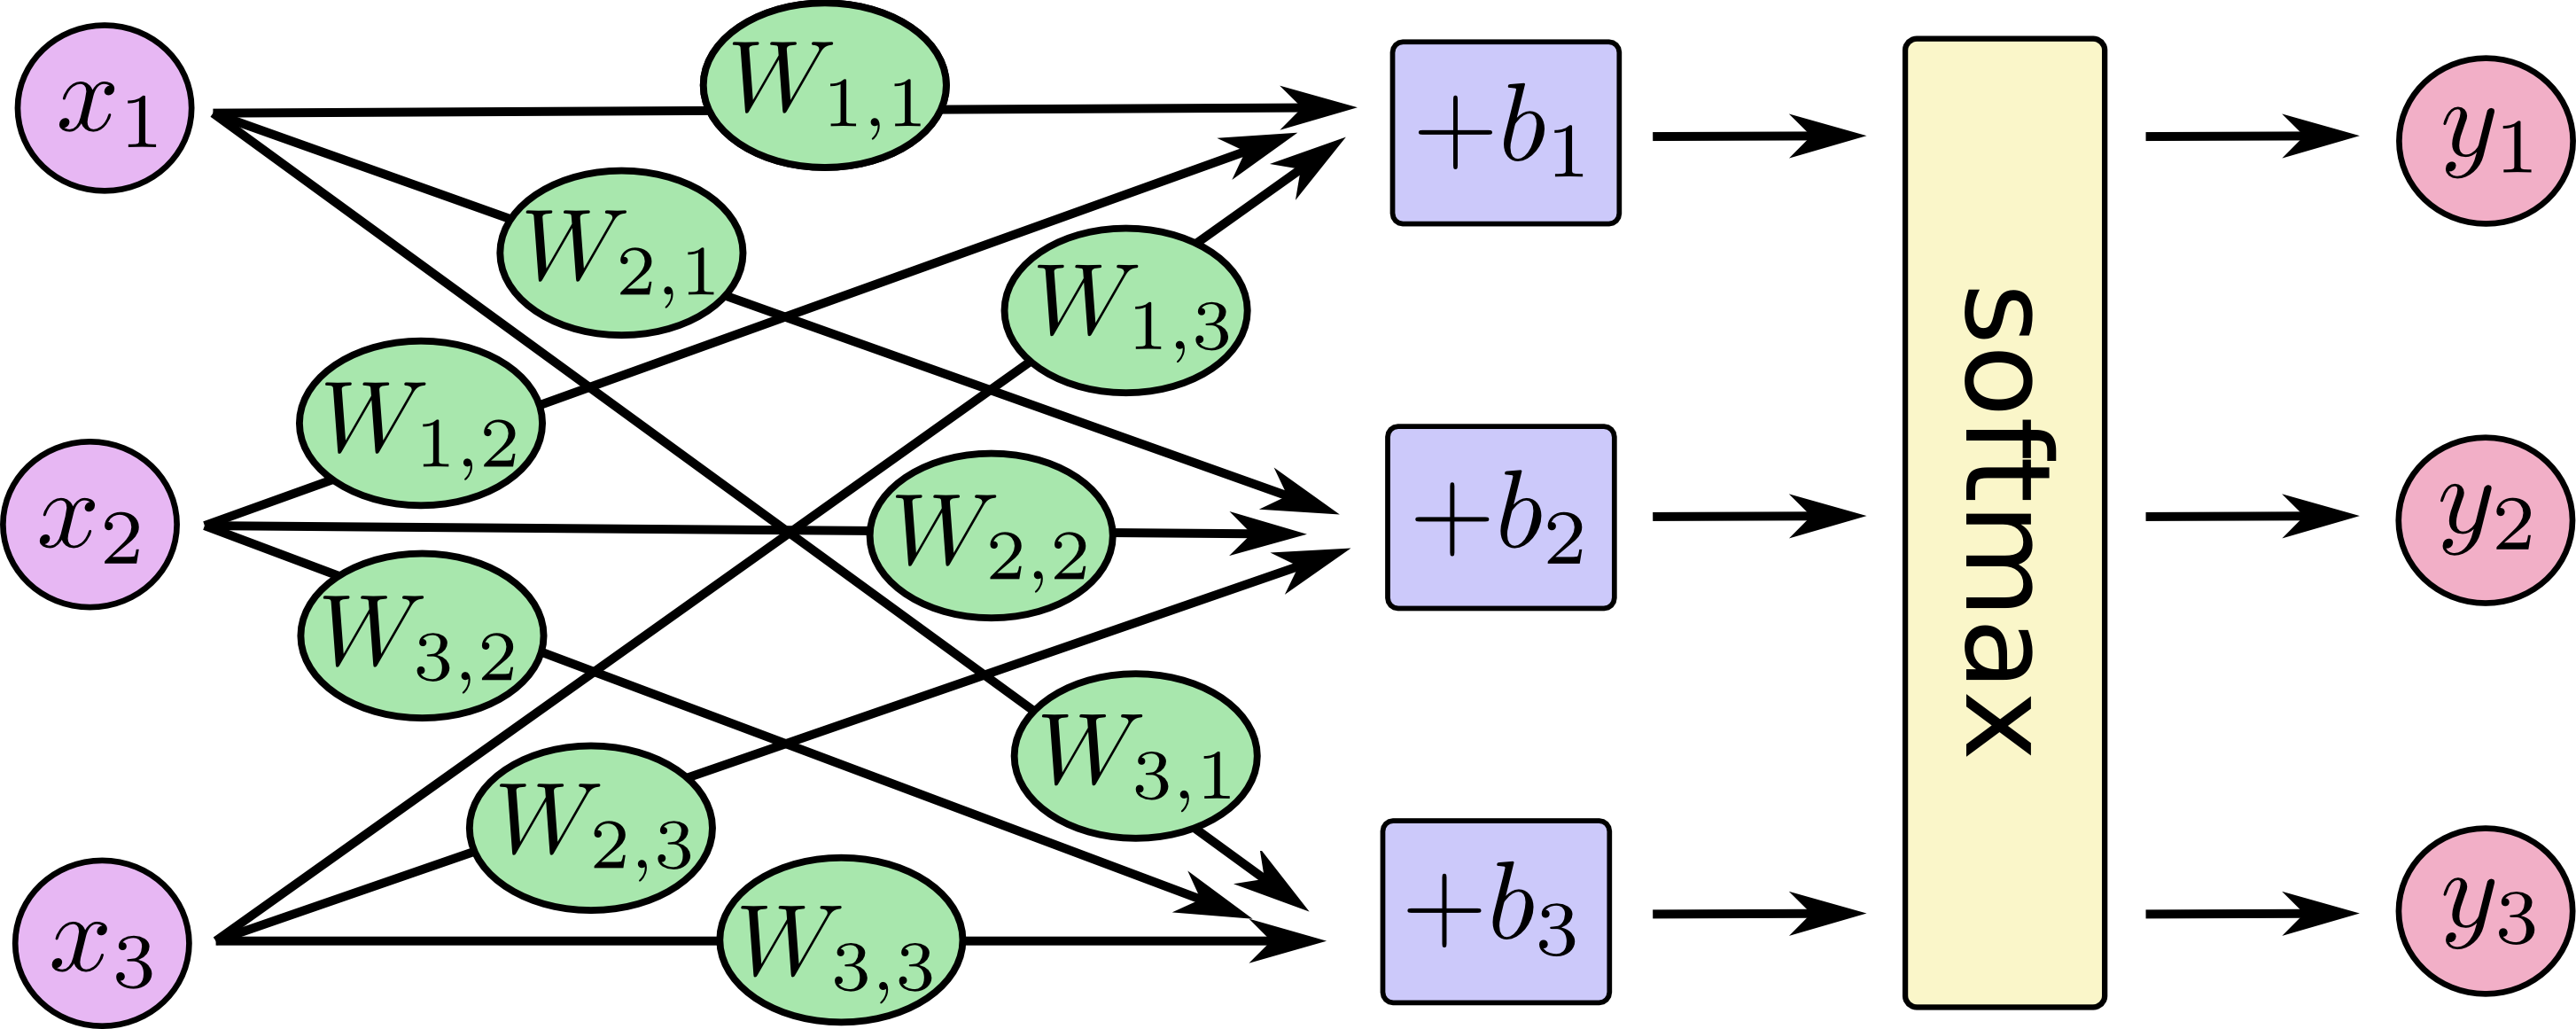
\includegraphics[width=.65\textwidth]{../SOURCE/images/softmax-regression-scalargraph.png}
\end{center}
如果把它写成一个方程,可以得到:
\begin{center}
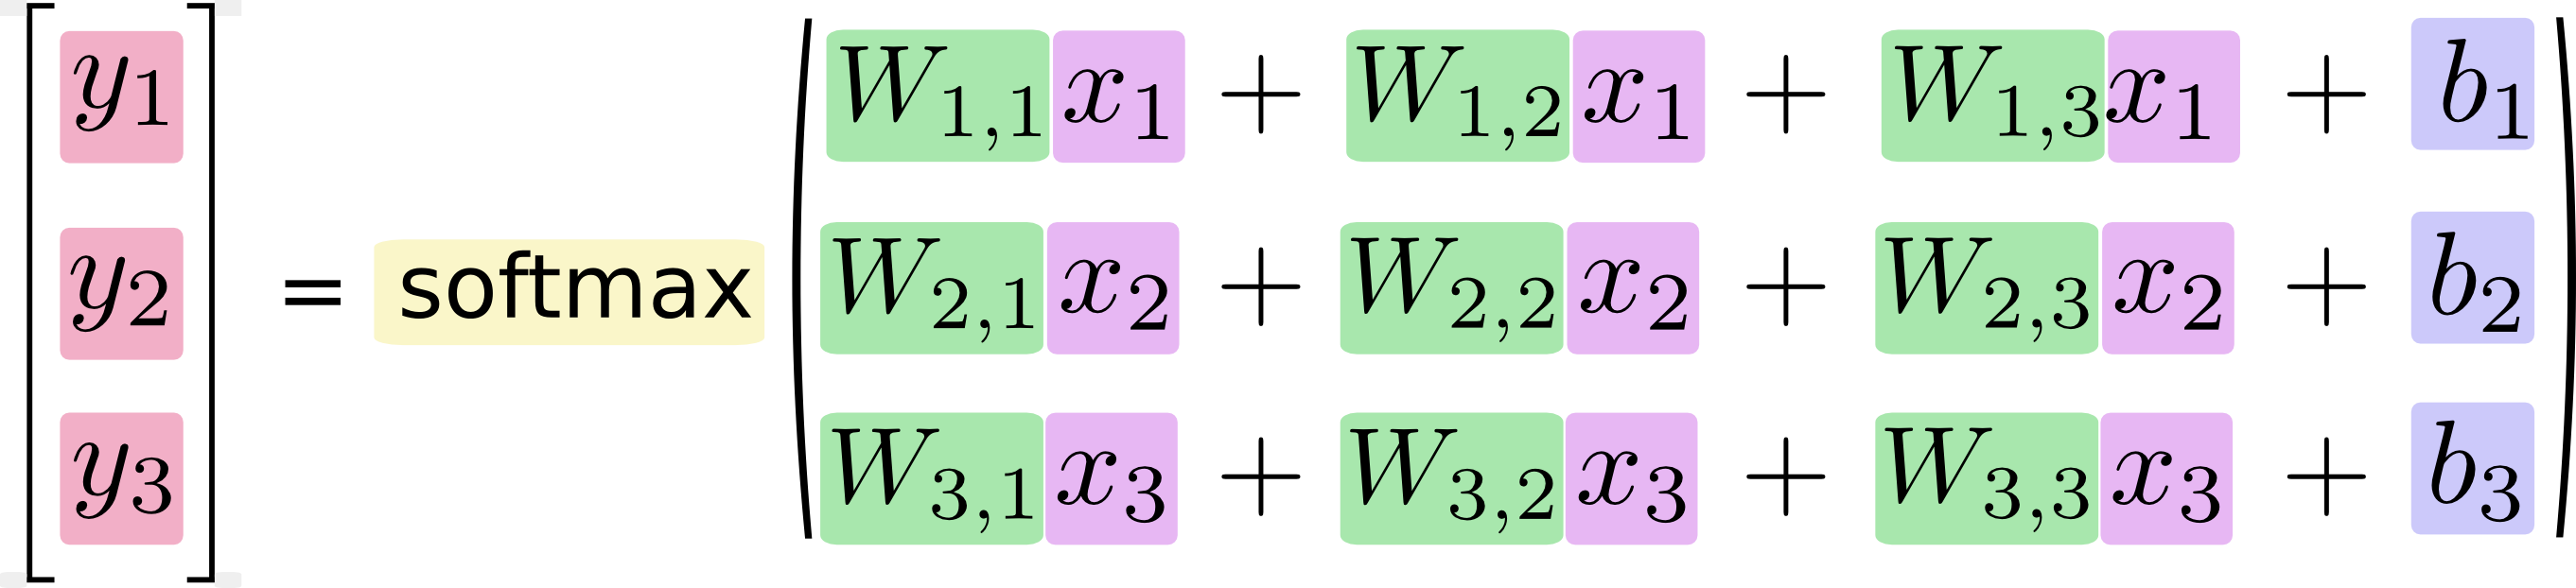
\includegraphics[width=.68\textwidth]{../SOURCE/images/softmax-regression-scalarequation.png}
\end{center}
我们也可以用向量表示这个计算过程:用矩阵乘法和向量相加。这有助于提高计算效率(也是一种更有效的思考方式)。
\begin{center}
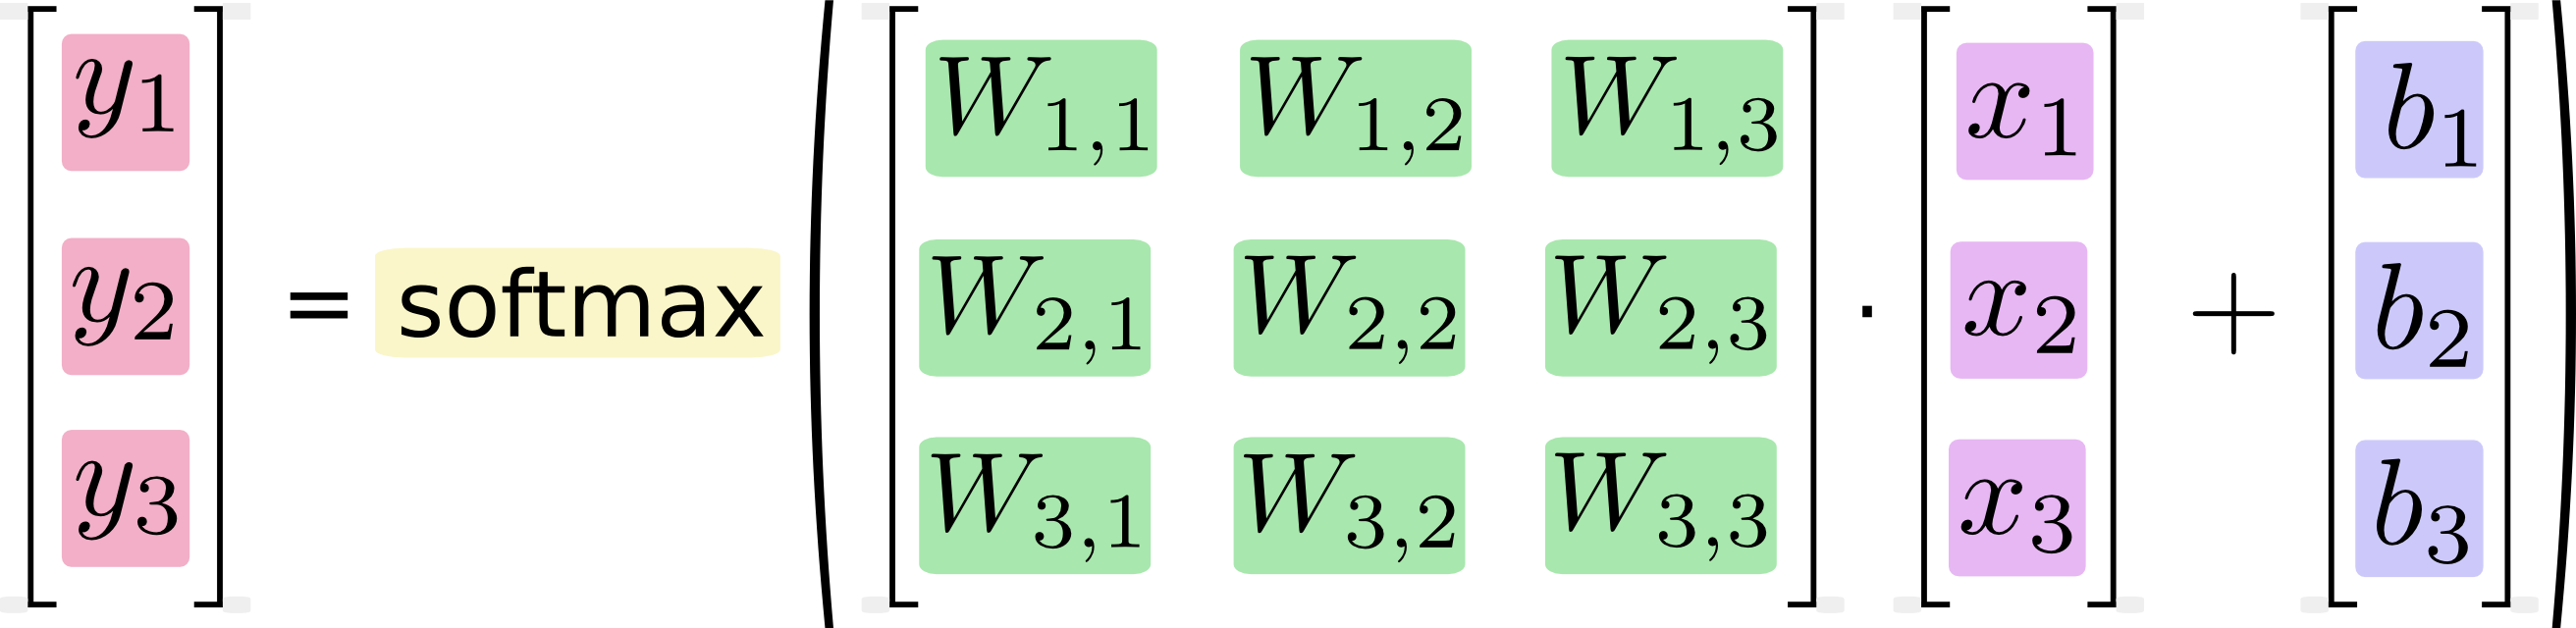
\includegraphics[width=.68\textwidth]{../SOURCE/images/softmax-regression-vectorequation.png}
\end{center}
更进一步,可以写成更加紧凑的方式:
\begin{equation}
y = softmax(W_x+b)
\end{equation}

\subsection {实现回归模型}
为了用python实现高效的数值计算,我们通常会使用函数库,比如NumPy,会把类似矩阵乘法这样的复杂运算使用其他外部语言实现。不幸的是,从外部计算切换回Python的每一个操作,仍然是一个很大的开销。如果你用GPU来进行外部计算,这样的开销会更大。用分布式的计算方式,也会花费更多的资源用来传输数据。

TensorFlow也把复杂的计算放在python之外完成,但是为了避免前面说的那些开销,它做了进一步完善。TensorFlow不单独地运行单一的复杂计算,而是让我们可以先用图描述一系列可交互的计算操作,然后全部一起在Python之外运行。(这样类似的运行方式,可以在不少的机器学习库中看到。)

使用TensorFlow之前,首先导入它:
\begin{lstlisting}
import tensorflow as tf
\end{lstlisting}
我们通过操作符号变量来描述这些可交互的操作单元,可以用下面的方式创建一个:
\begin{lstlisting}
x = tf.placeholder("float", [None, 784])
\end{lstlisting}
x 不是一个特定的值,而是一个占位符\lstinline{placeholder},我们在TensorFlow运行计算时输入这个值。我们希望能够输入任意数量的MNIST图像,每一张图展平成784维的向量。我们用2维的浮点数张量来表示这些图,这个张量的形状是 [None,784]。(这里的\lstinline{None}表示此张量的第一个维度可以是任何长度的。)

我们的模型也需要权重值和偏置量,当然我们可以把它们当做是另外的输入(使用占位符),但TensorFlow有一个更好的方法来表示它们:\lstinline{Variable}。 一个\lstinline{Variable}代表一个可修改的张量,存在在TensorFlow的用于描述交互性操作的图中。它们可以用于计算输入值,也可以在计算中被修改。对于各种机器学习应用,一般都会有模型参数,可以用\lstinline{Variable}表示。

\begin{lstlisting}
W = tf.Variable(tf.zeros([784,10]))
b = tf.Variable(tf.zeros([10]))
\end{lstlisting}

我们赋予\lstinline{tf.Variable} 不同的初值来创建不同的\lstinline{Variable}:在这里,我们都用全为零的张量来初始化\lstinline{W}和\lstinline{b}。因为我们要学习\lstinline{W}和\lstinline{b}的值,它们的初值可以随意设置。

注意,\lstinline{W}的维度是\lstinline{[784,10]},因为我们想要用784维的图片向量乘以它以得到一个10维的证据值向量,每一位对应不同数字类。\lstinline{b}的形状是\lstinline{[10]},所以我们可以直接把它加到输出上面。

现在,可以实现我们的模型了,只需以下一行代码:

\begin{lstlisting}
y = tf.nn.softmax(tf.matmul(x,W) + b)
\end{lstlisting}

首先,我们用\lstinline{tf.matmul(X,W)}表示$x$乘以$W$,对应之前等式里面的$W_x$,这里$x$是一个2维张量拥有多个输入。然后再加上$b$,把和输入到\lstinline{tf.nn.softmax}函数里面。

至此,我们先用了几行简短的代码来设置变量,然后只用了一行代码来定义我们的模型。TensorFlow不仅仅可以使softmax回归模型计算变得特别简单,它也用这种非常灵活的方式来描述其他各种数值计算,从机器学习模型对物理学模拟仿真模型。一旦被定义好之后,我们的模型就可以在不同的设备上运行:计算机的CPU,GPU,甚至是手机!

\subsection{训练模型}
为了训练我们的模型,我们首先需要定义一个指标来评估这个模型是好的。其实,在机器学习,我们通常定义指标来表示一个模型是坏的,这个指标称为成本(cost)或损失(loss),然后尽量最小化这个指标。但是,这两种方式是相同的。

一个非常常见的,非常漂亮的成本函数是“交叉熵”(cross-entropy)。交叉熵产生于信息论里面的信息压缩编码技术,但是它后来演变成为从博弈论到机器学习等其他领域里的重要技术手段。它的定义如下:
\begin{equation}
H_{y'}(u) = -\sum_i{y_{i'}log(y_i)}
\end{equation}
$y$是我们预测的概率分布,$y'$是实际的分布(我们输入的one-hot vector)。比较粗糙的理解是,交叉熵是用来衡量我们的预测用于描述真相的低效性。更详细的关于交叉熵的解释超出本教程的范畴,但是你很有必要好好理解它。

为了计算交叉熵,我们首先需要添加一个新的占位符用于输入正确值:
\begin{lstlisting}
y = tf.placeholder("float", [None,10])
\end{lstlisting}
然后我们可以用
\begin{equation}
-\sum{y'log(y)}
\end{equation}
计算交叉熵:

\begin{lstlisting}
cross_entropy = -tf.reduce_sum(y_*tf.log(y))
\end{lstlisting}

首先,用 tf.log 计算y的每个元素的对数。接下来,我们把y\_的每一个元素和tf.log(y\_)的对应元素相乘。最后,用tf.reduce\_sum计算张量的所有元素的总和。(注意,这里的交叉熵不仅仅用来衡量单一的一对预测和真实值,而是所有100幅图片的交叉熵的总和。对于100个数据点的预测表现比单一数据点的表现能更好地描述我们的模型的性能。

现在我们知道我们需要我们的模型做什么啦,用TensorFlow来训练它是非常容易的。因为TensorFlow拥有一张描述你各个计算单元的图,它可以自动地使用反向传播算法(backpropagation algorithm)来有效地确定你的变量是如何影响你想要最小化的那个成本值的。然后,TensorFlow会用你选择的优化算法来不断地修改变量以降低成本。

\begin{lstlisting}
train_step = tf.train.GradientDescentOptimizer(0.01).minimize(cross_entropy)
\end{lstlisting}

在这里,我们要求TensorFlow用梯度下降算法(gradient descent algorithm)以0.01的学习速率最小化交叉熵。梯度下降算法(gradient descent algorithm)是一个简单的学习过程,TensorFlow只需将每个变量一点点地往使成本不断降低的方向移动。当然TensorFlow也提供了其他许多优化算法:只要简单地调整一行代码就可以
使用其他的算法。

TensorFlow在这里实际上所做的是,它会在后台给描述你的计算的那张图里面增加一系列新的计算操作单元用于实现反向传播算法和梯度下降算法。然后,它返回给你的只是一个单一的操作,当运行这个操作时,它用梯度下降算法训练你的模型,微调你的变量,不断减少成本。

现在,我们已经设置好了我们的模型。在运行计算之前,我们需要添加一个操作来初始化我们创建的变量:

\begin{lstlisting}
init = tf.initialize_all_variables()
\end{lstlisting}

现在我们可以在一个 Session 里面启动我们的模型,并且初始化变量:
\begin{lstlisting}
sess = tf.Session()
sess.run(init)
\end{lstlisting}

然后开始训练模型,这里我们让模型循环训练1000次!
\begin{lstlisting}
for i in range(1000):
    batch_xs, batch_ys = mnist.train.next_batch(100)
    sess.run(train_step, feed_dict={x: batch_xs, y_: batch_ys})
\end{lstlisting}

该循环的每个步骤中,我们都会随机抓取训练数据中的100个批处理数据点,然后我们用这些数据点作为参数替换之前的占位符来运行train\_step。

使用一小部分的随机数据来进行训练被称为随机训练(stochastic training)- 在这里更确切的说是随机梯度下降训练。在理想情况下,我们希望用我们所有的数据来进行每一步的训练,因为这能给我们更好的训练结果,但显然这需要很大的计算开销。所以,每一次训练我们可以使用不同的数据子集,这样做既可以减少计算开销,又可以最大化地学习到数据集的总体特性。

\subsection{评估我们的模型}

那么我们的模型性能如何呢?

首先让我们找出那些预测正确的标签。\lstinline{tf.argmax()}是一个非常有用的函数,它能给你在一个张量里沿着某条轴的最高条目的索引值。比如,\lstinline{tf.argmax(y,1)}是模型认为每个输入最有可能对应的那些标签,而\lstinline{tf.argmax(y_,1)}代表正确的标签。我们可以用\lstinline{tf.equal} 来检测我们的预测是否真实标签匹配。

\begin{lstlisting}
correct_prediction = tf.equal(tf.argmax(y,1), tf.argmax(y_,1))
\end{lstlisting}

这行代码会给我们一组布尔值。为了确定正确预测项的比例,我们可以把布尔值转换成浮点数,然后取平均值。例如,\lstinline{[True, False, True, True]}会变成\lstinline{[1,0,1,1]},取平均值后得到 0.75 .

\begin{lstlisting}
accuracy = tf.reduce_mean(tf.cast(correct_prediction, "float"))
\end{lstlisting}

最后,我们计算所学习到的模型在测试数据集上面的正确率。

\begin{lstlisting}
print sess.run(accuracy, feed_dict={x: mnist.test.images, y_: mnist.test.labels})
\end{lstlisting}

最终结果值应该大约是91\%。

这个结果好吗?嗯,并不太好。事实上,这个结果是很差的。这是因为我们仅仅使用了一个非常简单的模型。不过,做一些小小的改进,我们就可以得到97\%的正确率。最好的模型甚至可以获得超过99.7\%的准确率!(想了解更多信息,可以看看这个关于各种模型的性能对比列表。)

比结果更重要的是,我们从这个模型中学习到的设计思想。不过,如果你仍然对这里的结果有点失望,可以查看下一个教程,在那里你将学到如何用FensorFlow构建更加复杂的模型以获得更好的性能!

原文地址:\href{http://tensorflow.org/tutorials/mnist/beginners/index.md}{MNIST For ML Beginners}
翻译:\href{https://github.com/linbojin}{linbojin} 校对:

%!TEX program = xelatex
% Encoding: UTF8
% SEIKA 2015


% Chapter 2 TutorialsHow to ...
% Section 2.3 minist pros

\newpage
\section {深入MNIST} \label{MINIST_pros}
TensorFlow是一个做大规模数值计算的强大库。其中一个特点就是它能够实现和训练深度神经网络。 在这一小节里,我们将会学习在MNIST上构建深度卷积分类器的基本步骤。

\emph{这个教程假设你已经熟悉神经网络和MNIST数据集。如果你尚未了解,请查看\hyperref[MINIST_beginner]{新手指南}.}

\subsection {安装}
在创建模型之前,我们会先加载MNIST数据集,然后启动一个TensorFlow的session。

\subsubsection {加载MINIST数据}

为了方便起见,我们已经准备了一个脚本来自动下载和导入MNIST数据集。它会自动创建一个'MNIST\_data'的目录来存储数据。

\begin{lstlisting}
import input_data
mnist = input_data.read_data_sets('MNIST_data', one_hot=True)
\end{lstlisting}

\subsubsection {开始TensorFlow的交互会话}

Tensorflow基于一个高效的C++模块进行运算。与这个模块的连接叫做session。一般而言,使用TensorFlow程序的流程是先创建一个图,然后在session中加载它。

这里,我们使用更加方便的InteractiveSession类。通过它,你可以更加灵活地构建你的代码。它能让你在运行图的时候,插入一些构建计算图的操作。这能给使用交互式文本shell如iPython带来便利。如果你没有使用InteractiveSession的话,你需要在开始session和加载图之前,构建整个计算图。

\begin{lstlisting}
import tensorflow as tf
sess = tf.InteractiveSession()
\end{lstlisting}

\subsubsection {计算图}

传统的计算行为中,为了更高效地在Python里进行数值计算,我们一般会使用像NumPy这样用其他语言编写的lib,在Python外完成这些费时的操作(例如矩阵运算)。可是,每一步操作依然会经常在Python和第三方lib之间切换。这些操作很糟糕,特别是当你想在GPU上进行计算,又或者想使用分布式的做法的时候。这些情况下数据传输代价高昂。

在TensorFlow中,也有Python与外界的频繁操作。但是它在这一方面,做了进一步的改良。TensorFlow构建一个交互操作的图,作为一个整体在Python外运行,而不是以代价高昂的单个交互操为单位在Python外运行。这与Theano、Torch的做法很相似。

所以,这部分Python代码,目的是构建这个在外部运行的计算图,并安排这个计算图的哪一部分应该被运行。详细请阅读计算图 部分的基本用法。 %add link here

\subsection{构建Softmax Regression模型}

在这小节里,我们将会构建一个一层线性的softmax regression模型。下一节里,我们会扩展到多层卷积网络。

\subsubsection{占位符}
我们先来创建计算图的输入(图片)和输出(类别)。

\begin{lstlisting}
x = tf.placeholder("float", shape=[None, 784])
y_ = tf.placeholder("float", shape=[None, 10])
\end{lstlisting}

这里的x和y并不是具体值,他们是一个placeholder,是一个变量,在TensorFlow运行计算的时候使用。

输入图片x是浮点数2维张量。这里,定义它的shape为[None, 784],其中784是单张展开的MNIST图片的维度数。shape的第一维输入指代一个batch的大小,None,可为任意值。输出值y\_也是一个2维张量,其中每一行为一个10维向量代表对应MNIST图片的分类。

虽然placeholder的shape参数是可选的,但有了它,TensorFlow能够自动捕捉因数据维度不一致导致的错误。

\subsubsection{Variables}

我们现在为模型定义权重W和偏置b。它们可以被视作是额外的输入量,但是TensorFlow有一个更好的方式来处理:Variable。一个Variable代表着在TensorFlow计算图中的一个值,它是能在计算过程中被读取和修改的。在机器学习的应用过程中,模型参数一般用Variable来表示。

\begin{lstlisting}
W = tf.Variable(tf.zeros([784,10]))
b = tf.Variable(tf.zeros([10]))
\end{lstlisting}

我们在调用tf.Variable的时候传入初始值。在这个例子里,我们把W和b都初始化为零向量。W是一个784x10的矩阵(因为我们有784个特征和10个输出值)。b是一个10维的向量(因为我们有10个分类)。

Variable需要在session之前初始化,才能在session中使用。初始化需要初始值(本例当中是全为零)传入并赋值给每一个Variable。这个操作可以一次性完成。

\begin{lstlisting}
sess.run(tf.initialize_all_variables())
\end{lstlisting}

\subsubsection{预测分类与损失函数}
现在我们可以实现我们的regression模型了。这只需要一行!我们把图片x和权重矩阵W相乘,加上偏置b,然后计算每个分类的softmax概率值。

\begin{lstlisting}
y = tf.nn.softmax(tf.matmul(x,W) + b)
\end{lstlisting}

在训练中最小化损失函数同样很简单。我们这里的损失函数用目标分类和模型预测分类之间的交叉熵。

\begin{lstlisting}
cross_entropy = -tf.reduce_sum(y_*tf.log(y))
\end{lstlisting}

注意,tf.reduce\_sum把minibatch里的每张图片的交叉熵值都加起来了。我们计算的交叉熵是指整个minibatch的。

\subsection{训练模型}

我们已经定义好了模型和训练的时候用的损失函数,接下来使用TensorFlow来训练。因为TensorFlow知道整个计算图,它会用自动微分法来找到损失函数对于各个变量的梯度。TensorFlow有大量内置的优化算法 这个例子中,我们用最速下降法让交叉熵下降,步长为0.01。

\begin{lstlisting}
train_step = tf.train.GradientDescentOptimizer(0.01).minimize(cross_entropy)
\end{lstlisting}

这一行代码实际上是用来往计算图上添加一个新操作,其中包括计算梯度,计算每个参数的步长变化,并且计算出新的参数值。

train\_step这个操作,用梯度下降来更新权值。因此,整个模型的训练可以通过反复地运行train\_step来完成。

\begin{lstlisting}
for i in range(1000):
    batch = mnist.train.next_batch(50)
    train_step.run(feed_dict={x: batch[0], y_: batch[1]})
\end{lstlisting}

每一步迭代,我们都会加载50个训练样本,然后执行一次train\_step,使用feed\_dict,用训练数据替换placeholder向量x和y\_。

注意,在计算图中,你可以用feed\_dict来替代任何张量,并不仅限于替换placeholder。

\subsubsection{评估模型}

我们的模型效果怎样?

首先,要先知道我们哪些label是预测正确了。tf.argmax是一个非常有用的函数。它会返回一个张量某个维度中的最大值的索引。例如,tf.argmax(y,1)表示我们模型对每个输入的最大概率分类的分类值。而 tf.argmax(y\_,1)表示真实分类值。我们可以用tf.equal来判断我们的预测是否与真实分类一致。

\begin{lstlisting}
correct_prediction = tf.equal(tf.argmax(y,1), tf.argmax(y_,1))
\end{lstlisting}

这里返回一个布尔数组。为了计算我们分类的准确率,我们将布尔值转换为浮点数来代表对、错,然后取平均值。例如:[True, False, True, True]变为[1,0,1,1],计算出平均值为0.75。

\begin{lstlisting}
accuracy = tf.reduce_mean(tf.cast(correct_prediction, "float"))
\end{lstlisting}

最后,我们可以计算出在测试数据上的准确率,大概是91\%。

\begin{lstlisting}
print accuracy.eval(feed_dict={x: mnist.test.images, y_: mnist.test.labels})
\end{lstlisting}

\subsection{构建多层卷积网络模型}

在MNIST上只有91\%正确率,实在太糟糕。在这个小节里,我们用一个稍微复杂的模型:卷积神经网络来改善效果。这会达到大概99.2\%的准确率。虽然不是最高,但是还是比较让人满意。

\subsubsection{权重初始化}

在创建模型之前,我们先来创建权重和偏置。一般来说,初始化时应加入轻微噪声,来打破对称性,防止零梯度的问题。因为我们用的是ReLU,所以用稍大于0的值来初始化偏置能够避免节点输出恒为0的问题(dead neurons)。为了不在建立模型的时候反复做初始化操作,我们定义两个函数用于初始化。

\begin{lstlisting}
def weight_variable(shape):
    initial = tf.truncated_normal(shape, stddev=0.1)
    return tf.Variable(initial)

def bias_variable(shape):
    initial = tf.constant(0.1, shape=shape)
    return tf.Variable(initial)
\end{lstlisting}

\subsubsection{卷积和池化}

TensorFlow在卷积和池化上有很强的灵活性。我们怎么处理边界?步长应该设多大?在这个实例里,我们会一直使用vanilla版本。我们的卷积使用1步长(stride size),0边距(padding size)的模板,保证输出和输入是同一个大小。我们的池化用简单传统的2x2大小的模板做max pooling。为了代码更简洁,我们把这部分抽象成一个函数。

\begin{lstlisting}
def conv2d(x, W):
    return tf.nn.conv2d(x, W, strides=[1, 1, 1, 1], padding='SAME')

def max_pool_2x2(x):
    return tf.nn.max_pool(x, ksize=[1, 2, 2, 1], strides=[1, 2, 2, 1], padding='SAME')
\end{lstlisting}

\subsubsection{第一层卷积}

现在我们可以开始实现第一层了。它由一个卷积接一个max pooling完成。卷积在每个5x5的patch中算出32个特征。权重是一个[5, 5, 1, 32]的张量,前两个维度是patch的大小,接着是输入的通道数目,最后是输出的通道数目。输出对应一个同样大小的偏置向量。

\begin{lstlisting}
W_conv1 = weight_variable([5, 5, 1, 32])
b_conv1 = bias_variable([32])
\end{lstlisting}

为了用这一层,我们把x变成一个4d向量,第2、3维对应图片的宽高,最后一维代表颜色通道。

\begin{lstlisting}
x_image = tf.reshape(x, [-1,28,28,1])
\end{lstlisting}

我们把x\_image和权值向量进行卷积相乘,加上偏置,使用ReLU激活函数,最后max pooling。

\begin{lstlisting}
h_conv1 = tf.nn.relu(conv2d(x_image, W_conv1) + b_conv1)
h_pool1 = max_pool_2x2(h_conv1)
\end{lstlisting}

\subsubsection{第二层卷积}

为了构建一个更深的网络,我们会把几个类似的层堆叠起来。第二层中,每个5x5的patch会得到64个特征。

\begin{lstlisting}
W_conv2 = weight_variable([5, 5, 32, 64])
b_conv2 = bias_variable([64])

h_conv2 = tf.nn.relu(conv2d(h_pool1, W_conv2) + b_conv2)
h_pool2 = max_pool_2x2(h_conv2)
\end{lstlisting}

\subsubsection{密集连接层}

现在,图片降维到7x7,我们加入一个有1024个神经元的全连接层,用于处理整个图片。我们把池化层输出的张量reshape成一些向量,乘上权重矩阵,加上偏置,使用ReLU激活。

\begin{lstlisting}
W_fc1 = weight_variable([7 * 7 * 64, 1024])
b_fc1 = bias_variable([1024])

h_pool2_flat = tf.reshape(h_pool2, [-1, 7*7*64])
h_fc1 = tf.nn.relu(tf.matmul(h_pool2_flat, W_fc1) + b_fc1)
\end{lstlisting}

\textbf{Dropout}

为了减少过拟合,我们在输出层之前加入dropout。我们用一个placeholder来代表一个神经元在dropout中被保留的概率。这样我们可以在训练过程中启用dropout,在测试过程中关闭dropout。 TensorFlow的tf.nn.dropout操作会自动处理神经元输出值的scale。所以用dropout的时候可以不用考虑scale。

\begin{lstlisting}
keep_prob = tf.placeholder("float")
h_fc1_drop = tf.nn.dropout(h_fc1, keep_prob)
\end{lstlisting}

\subsubsection{输出层}

最后,我们添加一个softmax层,就像前面的单层softmax regression一样。

\begin{lstlisting}
W_fc2 = weight_variable([1024, 10])
b_fc2 = bias_variable([10])

y_conv=tf.nn.softmax(tf.matmul(h_fc1_drop, W_fc2) + b_fc2)
\end{lstlisting}

\subsubsection{训练和评估模型}

这次效果又有多好呢?我们用前面几乎一样的代码来测测看。只是我们会用更加复杂的ADAM优化器来做梯度最速下降,在feed\_dict中加入额外的参数keep\_prob来控制dropout比例。然后每100次迭代输出一次日志。

\begin{lstlisting}
cross_entropy = -tf.reduce_sum(y_*tf.log(y_conv))
train_step = tf.train.AdamOptimizer(1e-4).minimize(cross_entropy)
correct_prediction = tf.equal(tf.argmax(y_conv,1), tf.argmax(y_,1))
accuracy = tf.reduce_mean(tf.cast(correct_prediction, "float"))
sess.run(tf.initialize_all_variables())
for i in range(20000):
  batch = mnist.train.next_batch(50)
  if i%100 == 0:
    train_accuracy = accuracy.eval(feed_dict={
        x:batch[0], y_: batch[1], keep_prob: 1.0})
    print "step %d, training accuracy %g"%(i, train_accuracy)
  train_step.run(feed_dict={x: batch[0], y_: batch[1], keep_prob: 0.5})

print "test accuracy %g"%accuracy.eval(feed_dict={
    x: mnist.test.images, y_: mnist.test.labels, keep_prob: 1.0})
\end{lstlisting}

以上代码,在最终测试集上的准确率大概是99.2%。

目前为止,我们已经学会了用TensorFlow来快速和简易地搭建、训练和评估一个复杂一点儿的深度学习模型。

原文地址:Deep MNIST for Experts
翻译:chenweican
校对:HongyangWang
%!TEX program = xelatex
% Encoding: UTF8
% SEIKA 2015


% Chapter 2 Tutorials
% Section 2.4 TensorFlow Mechanics 101


\newpage
\section {TensorFlow Mechanics 101} \label{tf_mech101}

代码地址: tensorflow/g3doc/tutorials/mnist/

本篇教程的目的,是向大家展示如何利用TensorFlow使用(经典)MNIST数据集训练并评估一个用于识别手写数字的简易前馈神经网络(feed-forward neural network)。我们的目标读者是有兴趣使用TensorFlow的机器学习资深人士。

因此,撰写该系列教程并不是为了教大家机器学习领域的基础知识。

在学习本教程之前,请确保您已按照安装TensorFlow教程中的要求,完成了安装。

\subsection {教程使用的文件}

本教程引用如下文件:

% add table here

只需要直接运行fully\_connected\_feed.py文件,就可以开始训练:

python fully\_connected\_feed.py

\subsection {准备数据}

MNIST是机器学习领域的一个经典问题,指的是让机器查看一系列大小为28x28像素的手写数字灰度图像,并判断这些图像代表0-9中的哪一个数字。

\begin{center}

\includegraphics[width=.55\textwidth]{../SOURCE/images/MNIST.png}
\end{center}

更多相关信息,请查阅Yann LeCun网站中关于MNIST的介绍 或者Chris Olah对MNIST的可视化探索。

\subsubsection{下载}

在`run\_training()`方法的一开始,`input\_data.read\_data\_sets()`函数会确保你的本地训练文件夹中,已经下载了正确的数据,然后将这些数据解压并返回一个含有`DataSet`实例的字典。

\begin{lstlisting}
data_sets = input_data.read_data_sets(FLAGS.train_dir, FLAGS.fake_data)
\end{lstlisting}\footnote{`fake\_data`标记是用于单元测试的,读者可以不必理会。}

% 数据集 | 目的
% --- | ---
% `data_sets.train` | 55000个图像和标签(labels),作为主要训练集。
% `data_sets.validation` | 5000个图像和标签,用于迭代验证训练准确度。
% `data_sets.test` | 10000个图像和标签,用于最终测试训练准确度(trained accuracy)。

Edit table here\footnote{了解更多数据有关信息,请查阅此系列教程的[数据下载](mnist/download/index.md)
部分.}

\subsubsection{输入与占位符}
% ### 输入与占位符(Inputs and Placeholders) <a class="md-anchor" id="AUTOGENERATED-inputs-and-placeholders"></a>

\lstinline{placeholder_inputs()}函数将生成两个\lstinline{tf.placeholder}
%[`tf.placeholder`](../api_docs/python/io_ops.md#placeholder)
操作,定义传入图表中的shape参数,shape参数中包括\lstinline{batch_size}值,后续还会将实际的训练用例传入图表。

\begin{lstlisting}
images_placeholder = tf.placeholder(tf.float32, shape=(batch_size, IMAGE_PIXELS))
labels_placeholder = tf.placeholder(tf.int32, shape=(batch_size))
\end{lstlisting}

在训练循环(training loop)的后续步骤中,传入的整个图像和标签数据集会被切片,以符合每一个操作所设置的 \lstinline{batch_size}值,占位符操作将会填补以符合这个\lstinline{batch_size}值。然后使用\lstinline{feed_dict}参数,将数据传入\lstinline{sess.run()}函数。

\subsection {构建图表 (Build the Graph)}
%## 构建图表 (Build the Graph)<a class="md-anchor" id="AUTOGENERATED-build-the-graph"></a>

在为数据创建占位符之后,就可以运行\lstinline{mnist.py}文件,经过三阶段的模式函数操作:\lstinline{inference()}, \lstinline{loss()\lstinline},和\lstinline{training()}。图表就构建完成了。

\begin{enumerate}

\item \lstinline{inference()} —— 尽可能地构建好图表,满足促使神经网络向前反馈并做出预测的要求。

\item \lstinline{loss()} —— 往inference图表中添加生成损失(loss)所需要的操作(ops)。

\item \lstinline{training()} —— 往损失图表中添加计算并应用梯度(gradients)所需的操作。
\end{enumerate}

\begin{center}
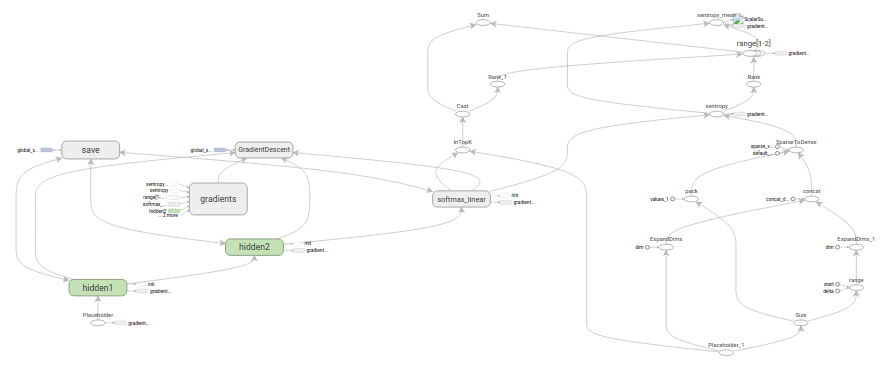
\includegraphics[width=.95\textwidth]{../SOURCE/images/mnist_subgraph.png}
\end{center}

\subsubsection{推理(Inference)}
%### 推理(Inference) <a class="md-anchor" id="AUTOGENERATED-inference"></a>

\lstinline{inference()}函数会尽可能地构建图表,做到返回包含了预测结果(output prediction)的Tensor。

它接受图像占位符为输入,在此基础上借助ReLu(Rectified Linear Units)激活函数,构建一对完全连接层(layers),以及一个有着十个节点(node)、指明了输出logtis模型的线性层。

每一层都创建于一个唯一的[`tf.name_scope`](../api_docs/python/framework.md#name_scope)之下,创建于该作用域之下的所有元素都将带有其前缀。

\begin{lstlisting}
with tf.name_scope('hidden1') as scope:
\end{lstlisting}

在定义的作用域中,每一层所使用的权重和偏差都在[`tf.Variable`](../api_docs/python/state_ops.md#Variable)实例中生成,并且包含了各自期望的shape。

\begin{lstlisting}
weights = tf.Variable(tf.truncated_normal([IMAGE_PIXELS, hidden1_units], stddev=1.0 / math.sqrt(float(IMAGE_PIXELS))), name='weights')
biases = tf.Variable(tf.zeros([hidden1_units]), name='biases')
\end{lstlisting}

例如,当这些层是在\lstinline{hidden1}作用域下生成时,赋予权重变量的独特名称将会是"\lstinline{hidden1/weights}"。

每个变量在构建时,都会获得初始化操作(initializer ops)。

在这种最常见的情况下,通过[`tf.truncated_normal`](../api_docs/python/constant_op.md#truncated_normal)函数初始化权重变量,给赋予的shape则是一个二维tensor,其中第一个维度代表该层中权重变量所连接(connect from)的单元数量,第二个维度代表该层中权重变量所连接到的(connect to)单元数量。对于名叫`hidden1`的第一层,相应的维度则是`[IMAGE_PIXELS, hidden1_units]`,因为权重变量将图像输入连接到了`hidden1`层。`tf.truncated_normal`初始函数将根据所得到的均值和标准差,生成一个随机分布。

然后,通过[`tf.zeros`](../api_docs/python/constant_op.md#zeros)函数初始化偏差变量(biases),确保所有偏差的起始值都是0,而它们的shape则是其在该层中所接到的(connect to)单元数量。

图表的三个主要操作,分别是两个[`tf.nn.relu`](../api_docs/python/nn.md#relu)操作,它们中嵌入了隐藏层所需的[`tf.matmul`](../api_docs/python/math_ops.md#matmul);以及logits模型所需的另外一个`tf.matmul`。三者依次生成,各自的`tf.Variable`实例则与输入占位符或下一层的输出tensor所连接。

\begin{lstlisting}
hidden1 = tf.nn.relu(tf.matmul(images, weights) + biases)
\end{lstlisting}

\begin{lstlisting}
hidden2 = tf.nn.relu(tf.matmul(hidden1, weights) + biases)
\end{lstlisting}

\begin{lstlisting}
logits = tf.matmul(hidden2, weights) + biases
\end{lstlisting}

最后,程序会返回包含了输出结果的`logits`Tensor。

\subsubsection{损失(Loss)}

\lstinline{loss()}函数通过添加所需的损失操作,进一步构建图表。

首先,\lstinline{labels_placeholer}中的值,将被编码为一个含有1-hot values的Tensor。例如,如果类标识符为“3”,那么该值就会被转换为:
\lstinline{[0, 0, 0, 1, 0, 0, 0, 0, 0, 0]}

\begin{lstlisting}
batch_size = tf.size(labels)
labels = tf.expand_dims(labels, 1)
indices = tf.expand_dims(tf.range(0, batch_size, 1), 1)
concated = tf.concat(1, [indices, labels])
onehot_labels = tf.sparse_to_dense(
    concated, tf.pack([batch_size, NUM_CLASSES]), 1.0, 0.0)
\end{lstlisting}

之后,又添加一个\lstinline{tf.nn.softmax_cross_entropy_with_logits}
%`](../api_docs/python/nn.md#softmax_cross_entropy_with_logits)
操作\footnote{交叉熵是信息理论中的概念,可以让我们描述如果基于已有事实,相信神经网络所做的推测最坏会导致什么结果。更多详情,请查阅博文《可视化信息理论》(http://colah.github.io/posts/2015-09-Visual-Information/)},用来比较\lstinline{inference()}函数与1-hot标签所输出的logits Tensor。

\begin{lstlisting}
cross_entropy = tf.nn.softmax_cross_entropy_with_logits(logits, onehot_labels, name='xentropy')
\end{lstlisting}

然后,使用\lstinline{tf.reduce_mean}
%(../api_docs/python/math_ops.md#reduce_mean)
函数,计算batch维度(第一维度)下交叉熵(cross entropy)的平均值,将将该值作为总损失。

\begin{lstlisting}
loss = tf.reduce_mean(cross_entropy, name='xentropy_mean')
\end{lstlisting}

最后,程序会返回包含了损失值的Tensor。

\subsubsection{训练}

\lstinline{training()}函数添加了通过梯度下降(gradient descent)将损失最小化所需的操作。

首先,该函数从\lstinline{loss()}函数中获取损失Tensor,将其交给\lstinline{[tf.scalar_summary]}
% ](../api_docs/python/train.md#scalar_summary)
,后者在与\lstinline{SummaryWriter}(见下文)配合使用时,可以向事件文件(events file)中生成汇总值(summary values)。在本篇教程中,每次写入汇总值时,它都会释放损失Tensor的当前值(snapshot value)。

\begin{lstlisting}
tf.scalar_summary(loss.op.name, loss)
\end{lstlisting}

接下来,我们实例化一个\lstinline{[tf.train.GradientDescentOptimizer]}
% (../api_docs/python/train.md#GradientDescentOptimizer)
,负责按照所要求的学习效率(learning rate)应用梯度下降法(gradients)。

\begin{lstlisting}
optimizer = tf.train.GradientDescentOptimizer(FLAGS.learning_rate)
\end{lstlisting}

之后,我们生成一个变量用于保存全局训练步骤(global training step)的数值,并使用\lstinline{[`minimize()`]}
% (../api_docs/python/train.md#Optimizer.minimize)
函数更新系统中的三角权重(triangle weights)、增加全局步骤的操作。根据惯例,这个操作被称为\lstinline{train_op},是TensorFlow会话(session)诱发一个完整训练步骤所必须运行的操作(见下文)。

\begin{lstlisting}
global_step = tf.Variable(0, name='global_step', trainable=False)
train_op = optimizer.minimize(loss, global_step=global_step)
\end{lstlisting}

最后,程序返回包含了训练操作(training op)输出结果的Tensor。

\subsection{训练模型}

一旦图表构建完毕,就通过\lstinline{fully_connected_feed.py}文件中的用户代码进行循环地迭代式训练和评估。

\subsubsection{图表 (The Graph)}

在\lstinline{run_training()}这个函数的一开始,是一个Python语言中的\lstinline{with}命令,这个命令表明所有已经构建的操作都要与默认的\lstinline{[`tf.Graph`]}
%(../api_docs/python/framework.md#Graph)
全局实例关联起来。

\begin{lstlisting}
with tf.Graph().as_default():
\end{lstlisting}

\lstinline{tf.Graph}实例是一系列可以作为整体执行的操作。TensorFlow的大部分场景只需要依赖默认图表一个实例即可。

利用多个图表的更加复杂的使用场景也是可能的,但是超出了本教程的范围。

\subsubsection{会话 (The Session)}

完成全部的构建准备、生成全部所需的操作之后,我们就可以创建一个\lstinline{[`tf.Session`]}
%(../api_docs/python/client.md#Session)
,用于运行图表。

\begin{lstlisting}
sess = tf.Session()
\end{lstlisting}

另外,也可以利用\lstinline{with}代码块生成\lstinline{Session},限制作用域:

\begin{lstlisting}
with tf.Session() as sess:
\end{lstlisting}

\lstinline{Session}函数中没有传入参数,表明该代码将会依附于(如果还没有创建会话,则会创建新的会话)默认的本地会话。

生成会话之后,所有\lstinline{tf.Variable}实例都会立即通过调用各自初始化操作中的\lstinline{[`sess.run()`]}
%(../api_docs/python/client.md#Session.run)
函数进行初始化。

\begin{lstlisting}
init = tf.initialize_all_variables()
sess.run(init)
\end{lstlisting}

\lstinline{[`sess.run()`]}
%(../api_docs/python/client.md#Session.run)
方法将会运行图表中与作为参数传入的操作相对应的完整子集。在初次调用时,\lstinline{init}操作只包含了变量初始化程序\lstinline{[`tf.group`]}
%(../api_docs/python/control_flow_ops.md#group)
。图表的其他部分不会在这里,而是在下面的训练循环运行。

\subsubsection{训练循环}

完成会话中变量的初始化之后,就可以开始训练了。

训练的每一步都是通过用户代码控制,而能实现有效训练的最简单循环就是:

\begin{lstlisting}
for step in xrange(max_steps):
    sess.run(train_op)
\end{lstlisting}

但是,本教程中的例子要更为复杂一点,原因是我们必须把输入的数据根据每一步的情况进行切分,以匹配之前生成的占位符。

\paragragh{向图表提}

执行每一步时,我们的代码会生成一个反馈字典(feed dictionary),其中包含对应步骤中训练所要使用的例子,这些例子的哈希键就是其所代表的占位符操作。

\lstinline{fill_feed_dict}函数会查询给定的\lstinline{DataSet},索要下一批次\lstinline{batch_size}的图像和标签,与占位符相匹配的Tensor则会包含下一批次的图像和标签。

\begin{lstlisting}
images_feed, labels_feed = data_set.next_batch(FLAGS.batch_size)
\end{lstlisting}

然后,以占位符为哈希键,创建一个Python字典对象,键值则是其代表的反馈Tensor。

\begin{lstlisting}
feed_dict = {
    images_placeholder: images_feed,
    labels_placeholder: labels_feed,
}
\end{lstlisting}

这个字典随后作为\lstinline{feed_dict}参数,传入\lstinline{sess.run()}函数中,为这一步的训练提供输入样例。

\paragragh{检查状态}

在运行\lstinline{sess.run}函数时,要在代码中明确其需要获取的两个值:\lstinline{`[train_op, loss]`}。

\begin{lstlisting}
for step in xrange(FLAGS.max_steps):
    feed_dict = fill_feed_dict(data_sets.train, images_placeholder, labels_placeholder)
    _, loss_value = sess.run([train_op, loss], feed_dict=feed_dict)
\end{lstlisting}

因为要获取这两个值,\lstinline{sess.run()}会返回一个有两个元素的元组。其中每一个\lstinline{Tensor}对象,对应了返回的元组中的numpy数组,而这些数组中包含了当前这步训练中对应Tensor的值。由于\lstinline{train_op}并不会产生输出,其在返回的元祖中的对应元素就是\lstinline{None},所以会被抛弃。但是,如果模型在训练中出现偏差,\lstinline{loss} Tensor的值可能会变成\lstinline{NaN},所以我们要获取它的值,并记录下来。

假设训练一切正常,没有出现\lstinline{NaN},训练循环会每隔100个训练步骤,就打印一行简单的状态文本,告知用户当前的训练状态。

\begin{lstlisting}
if step % 100 == 0:
    print 'Step %d: loss = %.2f (%.3f sec)' % (step, loss_value, duration)
\end{lstlisting}

\paragraph{状态可视化}
为了释放\lstinline{[TensorBoard]}
%(../how_tos/summaries_and_tensorboard.md)
所使用的事件文件(events file),所有的即时数据(在这里只有一个)都要在图表构建阶段合并至一个操作(op)中。

\begin{lstlisting}
summary_op = tf.merge_all_summaries()
\end{lstlisting}

在创建好会话(session)之后,可以实例化一个\lstinline{[`tf.train.SummaryWriter`]}
% (../api_docs/python/train.md#SummaryWriter)
,用于写入包含了图表本身和即时数据具体值的事件文件。

\begin{lstlisting}
summary_writer = tf.train.SummaryWriter(FLAGS.train_dir, graph_def=sess.graph_def)
\end{lstlisting}

最后,每次运行\lstinline{summary_op}时,都会往事件文件中写入最新的即时数据,函数的输出会传入事件文件读写器(writer)的\lstinline{add_summary()}函数。。

\begin{lstlisting}
summary_str = sess.run(summary_op, feed_dict=feed_dict)
summary_writer.add_summary(summary_str, step)
\end{lstlisting}

事件文件写入完毕之后,可以就训练文件夹打开一个TensorBoard,查看即时数据的情况。

\begin{center}
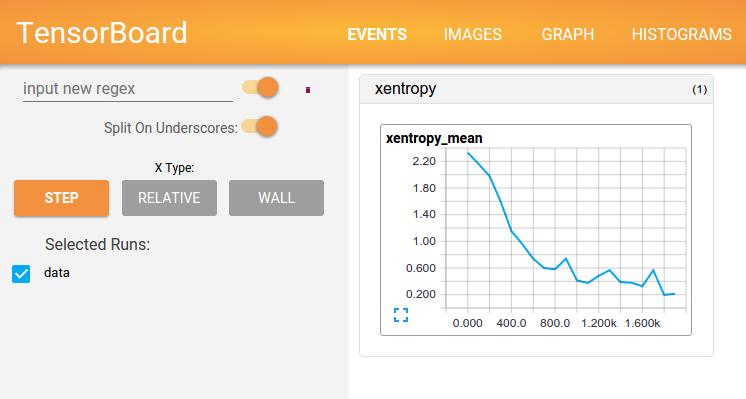
\includegraphics[width=.65\textwidth]{../SOURCE/images/mnist_tensorboard.png}
\end{center}

% ![MNIST TensorBoard](../images/mnist_tensorboard.png "MNIST TensorBoard")

**注意**:了解更多如何构建并运行TensorBoard的信息,请查看相关教程[Tensorboard:训练过程可视化](../how_tos/summaries_and_tensorboard.md)。

\aragraph{保存检查点(checkpoint)}

为了得到可以用来后续恢复模型以进一步训练或评估的检查点文件(checkpoint file),我们实例化一个\lstinline{[`tf.train.Saver`]}
% (../api_docs/python/state_ops.md#Saver)。

\begin{lstlisting}
saver = tf.train.Saver()
\end{lstlisting}

在训练循环中,将定期调用\lstinline{[`saver.save()`]}
%(../api_docs/python/state_ops.md#Saver.save)
方法,向训练文件夹中写入包含了当前所有可训练变量值得检查点文件。

\begin{lstlisting}
saver.save(sess, FLAGS.train_dir, global_step=step)
\end{lstlisting}

这样,我们以后就可以使用\lstinline{[`saver.restore()`]}
%(../api_docs/python/state_ops.md#Saver.restore)
方法,重载模型的参数,继续训练。

\begin{lstlisting}
saver.restore(sess, FLAGS.train_dir)
\end{lstlisting}

\subsection{评估模型}

每隔一千个训练步骤,我们的代码会尝试使用训练数据集与测试数据集,对模型进行评估。\lstinline{do_eval}函数会被调用三次,分别使用训练数据集、验证数据集合测试数据集。

\begin{lstlisting}
print 'Training Data Eval:'
do_eval(sess, eval_correct, images_placeholder, labels_placeholder, data_sets.train)
print 'Validation Data Eval:'
do_eval(sess, eval_correct, images_placeholder, labels_placeholder, data_sets.validation)
print 'Test Data Eval:'
do_eval(sess, eval_correct, images_placeholder, labels_placeholder, data_sets.test)
\end{lstlisting}

>注意,更复杂的使用场景通常是,先隔绝`data_sets.test`测试数据集,只有在大量的超参数优化调整(hyperparameter tuning)之后才进行检查。但是,由于MNIST问题比较简单,我们在这里一次性评估所有的数据。

\subsubsection {构建评估图表(Eval Graph)}

在打开默认图表(Graph)之前,我们应该先调用`get_data(train=False)`函数,抓取测试数据集。

\begin{lstlisting}
test_all_images, test_all_labels = get_data(train=False)
\end{lstlisting}

在进入训练循环之前,我们应该先调用`mnist.py`文件中的`evaluation`函数,传入的logits和标签参数要与`loss`函数的一致。这样做事为了先构建Eval操作。

\begin{lstlisting}
eval_correct = mnist.evaluation(logits, labels_placeholder)
\end{lstlisting}

`evaluation`函数会生成[`tf.nn.in_top_k`](../api_docs/python/nn.md#in_top_k)
操作,如果在K个最有可能的预测中可以发现真的标签,那么这个操作就会将模型输出标记为正确。在本文中,我们把K的值设置为1,也就是只有在预测是真的标签时,才判定它是正确的。

\begin{lstlisting}
eval_correct = tf.nn.in_top_k(logits, labels, 1)
\end{lstlisting}

\subsubsection {评估图表的输出(Eval Output)}

之后,我们可以创建一个循环,往其中添加`feed_dict`,并在调用`sess.run()`函数时传入`eval_correct`操作,目的就是用给定的数据集评估模型。

\begin{lstlisting}
for step in xrange(steps_per_epoch):
    feed_dict = fill_feed_dict(data_set,
                               images_placeholder,
                               labels_placeholder)
    true_count += sess.run(eval_correct, feed_dict=feed_dict)
\end{lstlisting}

`true_count`变量会累加所有`in_top_k`操作判定为正确的预测之和。接下来,只需要将正确测试的总数,除以例子总数,就可以得出准确率了。

\begin{lstlisting}
precision = float(true_count) / float(num_examples)
print '  Num examples: %d  Num correct: %d  Precision @ 1: %0.02f' % (
    num_examples, true_count, precision)
\end{lstlisting}

> 原文:[TensorFlow Mechanics 101](http://www.tensorflow.org/tutorials/mnist/tf/index.md)
> 翻译:[bingjin](https://github.com/bingjin)
> 校对:[LichAmnesia](https://github.com/LichAmnesia)
%!TEX program = xelatex
% Encoding: UTF8
% SEIKA 2015


% Chapter 2 Tutorials
% Section 2.5


\newpage
\section {卷积神经网络} \label{cnn}

\subsection {Overview}

%Ⓔ CIFAR-10 classification is a common benchmark problem in machine learning. The problem is to classify RGB 32x32 pixel images across 10 categories: airplane, automobile, bird, cat, deer, dog, frog, horse, ship, and truck.

对CIFAR-10 数据集的分类是机器学习中一个公开的基准测试问题,其任务是对一组32x32RGB的图像进行分类,这些图像涵盖了10个类别:\lstinline{airplane}, \lstinline{automobile}, \lstinline{bird}, \lstinline{cat}, \lstinline{deer}, \lstinline{dog}, \lstinline{frog}, \lstinline{horse}, \lstinline{ship}, 和 \lstinline{truck}.\footnote{This tutorial is intended for advanced users of TensorFlow and assumes expertise and experience in machine learning}

\begin{center}
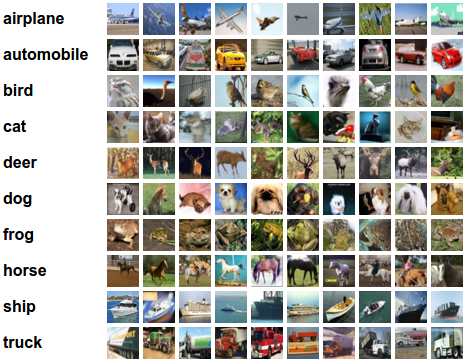
\includegraphics[width=.7\textwidth]{../SOURCE/images/cifar_samples.png}
\end{center}

想了解更多信息请参考\href{http://www.cs.toronto.edu/~kriz/cifar.html}{CIFAR-10 page},以及Alex Krizhevsky写的\href{http://www.cs.toronto.edu/~kriz/learning-features-2009-TR.pdf}{技术报告}。

\subsubsection {目标}
本教程的目标是建立一个用于识别图像的相对较小的卷积神经网络,在这一过程中,本教程会:

\begin{itemize}
\item 着重于建立一个规范的网络组织结构,训练并进行评估;
\item 为建立更大规模更加复杂的模型提供一个范例
\end{itemize}

选择CIFAR-10是因为它的复杂程度足以用来检验TensorFlow中的大部分功能,并可将其扩展为更大的模型。与此同时由于模型较小所以训练速度很快,比较适合用来测试新的想法,检验新的技术。

\subsubsection {本教程的重点}
CIFAR-10 教程演示了在TensorFlow上构建更大更复杂模型的几个种重要内容:

\begin{itemize}
\item 相关核心数学对象,如卷积、修正线性激活、最大池化以及局部响应归一化;
\item 训练过程中一些网络行为的可视化,这些行为包括输入图像、损失情况、网络行为的分布情况以及梯度;
\item 算法学习参数的移动平均值的计算函数,以及在评估阶段使用这些平均值提高预测性能;
\item 实现了一种机制,使得学习率随着时间的推移而递减;
\item 为输入数据设计预存取队列,将磁盘延迟和高开销的图像预处理操作与模型分离开来处理;
\end{itemize}

我们也提供了模型的多GUP版本,用以表明:

\begin{itemize}
\item 可以配置模型后使其在多个GPU上并行的训练
\item 可以在多个GPU之间共享和更新变量值
\end{itemize}

我们希望本教程给大家开了个头,使得在Tensorflow上可以为视觉相关工作建立更大型的Cnns模型

\subsubsection {模型架构}

本教程中的模型是一个多层架构,由卷积层和非线性层(nonlinearities)交替多次排列后构成。这些层最终通过全连通层对接到softmax分类器上。这一模型除了最顶部的几层外,基本跟Alex Krizhevsky提出的模型一致。

在一个GPU上经过几个小时的训练后,该模型达到了最高86\%的精度。细节请查看下面的描述以及代码。模型中包含了1,068,298个学习参数,分类一副图像需要大概19.5M个乘加操作。

\subsection {Code Organization}

本教程的代码位于\href{https://tensorflow.googlesource.com/tensorflow/+/master/tensorflow/models/image/cifar10/}{tensorflow/models/image/cifar10/}.

% insert table here

\subsection {CIFAR-10 模型}


\subsubsection {Model Inputs}

\subsubsection {Model Prediction}

\subsubsection {Model Training}

\subsection {Lauching and Training the Model}

\subsection {Evaluating a Model}

\subsection {Traning a Model Using Multiple GPU Cards}

\subsubsection {Placing Variables and Operations on Devices}

\subsubsection {Lauching and Training the Model on Multiple GPU cards}

\subsection {Next Steps}





% \newpage
% \section {TensorFlow运作方式}
% \section {卷积神经网络}
% \subsection {概述}
% \subsection {代码组织}
% \subsection {CIFAR-10模型}_
% \subsection {开始执行并训练模型}
% \subsection {模型评估}
% \section {Vector Representations of Words}
% \section {循环神经网络}
% \section {曼德博(Mandelbrot)集合}
% \section {偏微分方程}
% \section {MNIST数据集下载}


\newpage
% Chapter 3 How to...
% 第三章 运作方式
%!TEX program = xelatex
% Encoding: UTF8
% SEIKA 2015


% Chapter 3 How to ...
% Section 3.1

\chapter{运作方式}

\section{变量:创建、初始化、保存和加载}

当训练模型时,用变量来存储和更新参数。变量包含张量 (Tensor)存放于内存的缓存区。建模时它们需要被明确地初始化,模型训练后它们必须被存储到磁盘。这些变量的值可在之后模型训练和分析是被加载。

本文档描述以下两个TensorFlow类。点击以下链接可查看完整的API文档:
\begin{itemize}
  \item tf.Variable 类 % add link here
  \item tf.train.Saver 类 % add link here
\end{itemize}

\subsection {创建}

当创建一个变量时,你将一个张量作为初始值传入构造函数Variable()。TensorFlow提供了一系列操作符来初始化张量,初始值是常量或是随机值。
% add link here

\begin{lstlisting}
# Create two variables.
weights = tf.Variable(tf.random_normal([784, 200], stddev=0.35), name="weights")
biases = tf.Variable(tf.zeros([200]), name="biases")
\end{lstlisting}

调用tf.Variable()添加一些操作(Op, operation)到graph:
\begin{itemize}
  \item 一个Variable操作存放变量的值。
  \item 一个初始化op将变量设置为初始值。这事实上是一个tf.assign操作。
  \item 初始值的操作,例如示例中对biases变量的zeros操作也被加入了graph。
\end{itemize}
tf.Variable的返回值是Python的tf.Variable类的一个实例。

\subsection {初始化}

变量的初始化必须在模型的其它操作运行之前先明确地完成。最简单的方法就是添加一个给所有变量初始化的操作,并在使用模型之前首先运行那个操作。

你或者可以从检查点文件中重新获取变量值,详见下文。

使用tf.initialize\_all\_variables()添加一个操作对变量做初始化。记得在完全构建好模型并加载之后再运行那个操作。
% \input{how_tos/sec_1_variables}


\newpage
\chapter{资源}

\newpage
\chapter{其他}

\end{document}